\documentclass[letterpaper]{article}
\usepackage{natbib}
% \usepackage[colorinlistoftodos]{todonotes}
\usepackage[margin=1.05in]{geometry} %Margins
\usepackage[utf8]{inputenc}
\usepackage{amsmath,amssymb,amsfonts,amsthm} %Ams Math
\usepackage{enumerate}
\usepackage{pgf, tikz}
\usepackage{subfig} % For subfigures in plots
\usetikzlibrary{positioning}
\usepackage{hyperref}
\usepackage[capitalize]{cleveref}
\usetikzlibrary{arrows, automata}
\usepackage{algpseudocode}
\usepackage{algorithm}
\usepackage{bbm}
\usepackage{nth}
\algnewcommand\algorithmicforeach{\textbf{for each:}}
\algnewcommand\ForEach{\item[ \algorithmicforeach]}

% Proposition Environments:
    \newtheorem{proposition}{Proposition}
    \newtheorem{theorem}{Theorem}
    \newtheorem*{proposition*}{Proposition}
    \newtheorem{lemma}{Lemma}
    \newtheorem{property}{Property}
    \newtheorem{claim}{Claim}
    \newtheorem{corollary}{Corollary}
    \newtheorem{conjecture}{Conjecture}
    \newtheorem{observation}{Observation}
    \newtheorem{definition}{Definition} \theoremstyle{definition} 

\let\ringaccent\r % We need this to make the swedish a with the circle on it, since that command is normally given by \r, which we are now using for a bold vector.
\def\x*{\mathbf{x^*}}
\def\x{\mathbf{x}}
\def\v{\mathbf{v}}
\def\px{\mathbf{\pi}}
\def\px*{\mathbf{\pi^*}}
\def\lx{\mathbf{\lambda}}
\def\q{\mathbf{q}}
\def\w{\mathbf{w}}
\def\y{\mathbf{y}}
\def\z{\mathbf{z}}
\def\b{\mathbf{b}}
\def\c{\mathbf{c}}
\def\e{\mathbf{e}}
\def\0{\mathbf{0}}
\def\1{\mathbf{1}}
\def\r{\mathbf{r}}

\def\cC{{\cal{C}}}

 % Commands for adding notes from Jim, Nate, or Scott,
 % followed by commands for removing the notes

 %Dorit inserted another version

\newcommand{\SG}[1]{\textbf{\color{red}SG: #1}}
\newcommand{\NA}[1]{\textbf{\color{cyan}NA: #1}}
\newcommand{\jnote}[1]{\textbf{\color{teal}JO: #1}}
\newcommand{\DO}[1]{\textbf{\color{blue}DH: #1}}

\newcommand{\taba}{\hspace*{0.25in}}
\newcommand{\tabb}{\hspace*{.5in}}
\newcommand{\tabc}{\hspace*{.75in}}
\newcommand{\tabd}{\hspace*{1in}}


   \usepackage{xcolor}
    % \newcommand\jnote[1]{\textcolor{red}{#1}}
    %\renewcommand\jnote[1]{}
    \newcommand\nnote[1]{\textcolor{green}{#1}}
    %\renewcommand\nnote[1]{}
    \newcommand\snote[1]{\textcolor{blue}{#1}}
    %\renewcommand\snote[1]{}

 
 
\title{The Strong Maximum Circulation Algorithm: A New Method for Aggregating Preference Rankings}



\author{Nathan Atkinson \\ University of Wisconsin \\ \tt{natkinson@wisc.edu}  \and Scott C. Ganz \\  Georgetown MSB and AEI \\ \tt{scott.ganz@georgetown.edu} \and Dorit S. Hochbaum \\ UC Berkeley \\ \tt{dhochbaum@berkeley.edu} \and James B. Orlin \\ MIT Sloan \\ \tt{jorlin@mit.edu}}



\begin{document}
\date{}
\maketitle

\begin{abstract}
We present a new optimization-based method for aggregating preferences in settings where each decision maker, or voter, expresses preferences over pairs of alternatives, or votes. The challenge is to determine a ranking that summarizes the voters' preferences in cases when some of the votes conflict. Only a collection of votes that contains no cycles represents a consensus partial order over alternatives. Our approach to identifying a consensus partial order is motivated by the observation that a collection of votes that form a cycle can be treated as collective ties. The approach is then to remove unions of cycles of votes, or circulations, from the vote graph and determine aggregate preferences from the remainder.

We study the removal of \emph{maximal circulations} attained by any union of cycles the removal of which leaves an acyclic graph. We establish that the removal of a maximal circulation results in non-unique and conflicting partial orders.  Moreover, we prove that a {\em minimum maximal} circulation---i.e., a maximal circulation containing smallest number of votes---is an NP-hard problem. 

Instead, we introduce the \textit{strong maximum circulation}, the removal of which guarantees a {\bf unique} outcome in terms of the induced partial order, called the \textit{strong partial order}. The strong partial order includes the aggregate preferences induced by the removal of any maximum circulation. In that sense, conditional on removing a circulation containing as many votes as possible, the strong partial order maximizes the number of induced aggregate preferences over pairs of alternatives. The strong maximum circulation also satisfies strong complementary slackness conditions, and is shown here to be solved efficiently as a network flow problem. We further establish the relationship between the dual of the maximum circulation problem and Kemeny's method, a popular optimization-based approach for preference aggregation. 


%Furthermore, the strong partial order includes all preferences for which there exists a maximum circulation that does not include that preference.  In that sense the strong partial order results from the removal of smallest number of preferences.  


%We further establish that the removal of a maximal circulation results in non-unique and conflicting partial orders.  Moreover, we prove that a {\em minimum maximal} circulation, that removes the smallest number of votes, is an NP-hard problem. 

%Furthermore, it contains all of the aggregate preferences remaining following the elimination of \textit{any} maximum circulation. In contrast, the well-known, optimization-based, Kemeny method, that removes a minimum number of votes so the remaining graph is acyclic, has non-unique output and can return multiple, conflicting optimal rankings for the same input. Furthermore, Kemeny's method requires solving an NP-hard problem, whereas our algorithm is efficient, based on network flow techniques, and runs in strongly polynomial time, independent of the number of votes.

%We address the construction of a consistent ranking from the partial order and show that rankings based on a convex relaxation of Kemeny's model are consistent with our partial order.  We then study the properties of removing a \emph{maximal circulation} versus a \emph{maximum circulation} and establish that, while maximal circulations will in general identify a larger number of aggregate preferences than maximum circulations, the partial orders induced by the removal of different maximal circulations are not unique and may be conflicting.  Moreover, finding a {\em minimum maximal} circulation, that removes the smallest number of votes, is an NP-hard problem. \DO{not a good way to conclude the abstract - on a negative note, of what CANNOT be done.}

\end{abstract}

\bigskip

% \section*{General comments:}
% \NA{Reviewer 4 wanted us to comment on why eliminating fractional votes is also reasonable. I think that the fact that we show that the strong partial order is the union of partial orders induced by any maximum circulation is a good justification for this. But consider whether we should add additional justification.}

% \NA{ Reviewer 3 wants more on ``why maximum''  rather than a different maximal circulation, and given that, ``why strong maximum''. Given that we conver the extremes of maximum and minimum, I don't know what else we should say. Perhaps this can be addressed in the conclusion by alluding to the possibility of other cycle removal approaches. I added a few sentences there.}

% \SG{I've tried to further simplify the introduction. I've also tried to deemphasize the contrast with Kemeny's method in our discussion of cycle removal approaches. I may be wrong -- Dorit, please let me know if I am! -- but I suspect that reviewers at this journal will not be immediately familiar with Kemeny's method. If so, it seems sufficient to say that Kemeny's method is popular and that it has the stated drawbacks without spending valuable real estate in the introduction on the Kemeny example. We still have the detailed illustrative example of the SMC algorithm, which I think suffices.}

\section{Introduction}

The problem of aggregating preferences is of central interest to a broad set of problems in economics, political science, psychology, operations research, and computer science. Given a set of (possibly conflicting) pairwise comparisons of alternatives, how can we determine non-conflicting aggregate pairwise comparisons that best summarize the original data? This question is fundamental to topics as diverse as the analysis of democratic voting systems, the design of online search and recommendation algorithms, and the construction of nonparametric statistical tests.

It is well-known that no preference aggregation method satisfies every potential desirable normative property---e.g., non-dictatorship, independence of irrelevant alternatives, and Pareto efficiency \citep{arrow_social_1951,pini2009aggregating}. Further, existing approaches that are based on maximizing the alignment of an aggregate ranking with a set of pairwise comparisons face issues related to computational complexity that are driven by the exponential size of the set of possible orderings of alternatives \citep{bartholdi_voting_1989, fischer2016weighted}. As a result, there has been significant interest in applying approaches from optimization and machine learning in order to discover new aggregation methods that are both well-justified normatively and computationally efficient \citep[see, e.g.,][]{agarwal_mathematics_2010}.

We introduce a new optimization-based approach for aggregating preferences that is based on the logic of removing cycles of votes, i.e., sets of votes for which every vote in favor of an alternative is counterbalanced by a vote against that alternative. Given a cyclic set of votes, there is no principled way of saying that any alternative is preferred to any other. This insight points to the possibility of treating cycles of votes as uninformative ties and using the non-conflicting remainder to determine an aggregate preference ranking.

We represent a set of voters' pairwise preferences over alternatives, or votes, in a vote graph. The nodes of the vote graph are the alternatives.  For each pair of alternatives $i$ and $j$, we let $q_{ij}$ denote the number of voters who prefer $i$ to $j$.  An arc $(i, j)$ is in the vote graph provided that $q_{ij}>0$. The collection of votes is said to be \emph{conflicting} if there is a directed cycle in the vote graph. A set of votes is \emph{non-conflicting} if there is no directed cycle in the vote graph. For non-conflicting sets of votes, there is an induced partial order in which alternative $i$ is preferred to alternative $j$ if and only if there is a directed path from $i$ to $j$ in the vote graph.  This partial order is the smallest one that is consistent with the votes.

%Our approach is to remove cycles of votes from the vote graph and determine aggregate preferences from the non-conflicting remainder. %In that sense, following \cite{saari_capturing_2003}, our approach is to remove ties and declare the remaining non-conflicting votes as representing the ``voters' will'' (p. 342).

%THIS TEXT JUST HANGS HERE WITHOUT CONTEXT. Our method identifies cycles that create inconsistencies in the vote graph and eliminates them.  %When the original preference data are non-conflicting, our method recognizes the consistency and eliminates no votes.  When the original preference data is conflicting, our method will eliminate certain votes so that the remaining votes are non-conflicting.

% The most well-known vote elimination method is due to \citet{kemeny_mathematics_1959}.  Kemeny’s method is to remove the fewest number of votes so that the remaining set of votes is non-conflicting. While Kemeny's method has some nice theoretical properties, e.g., it can be justified in terms of minimizing the swap distance from the individual rankings \citep{brandt_rationalizations_2016}, it also suffers important drawbacks. First, Kemeny’s optimization model is equivalent to the NP-hard minimum feedback arc set (FAS) problem \citep{garyjohnson,bartholdi_voting_1989}.  Second, there may be alternative (conflicting) optimal solutions. That is, one optimal solution may have alternative $i$ preferred to alternative $j$ while a second optimal solution has alternative $j$ preferred to alternative $i$. This is called the \emph{paradox of Kemeny} \citep{muravyov_dealing_2014, yoo_new_2021}. These problems, which also plague similar preference aggregation methods that are justified by a vote-editing logic, also mean that one cannot efficiently determine whether a candidate ranking is optimal, whether a given set of votes has a unique optimal solution, or whether all of the optimal rankings have been enumerated \citep[see, e.g.,][]{fischer2016weighted}.



% The paradox of Kemeny is best illustrated when the vote graph consists of a single cycle, e.g., consider two votes on two alternatives, $1$ and $2$, with the corresponding graph depicted in Figure \ref{fig:cycle-a}. One vote states that $1$ is preferred to $2$, and the other vote states that $2$ is preferred to $1$. This graph contains two arcs $(1,2)$ and $(2,1)$, which together form a cycle 1-2-1. Obviously, there is no solution that agrees with both of these votes. 

%The solution where 1 is preferred to 2, $1\succ 2$, eliminates one vote: the vote $(2,1)$. The solution where 2 is preferred to 1, $2\succ 1$, also eliminates one vote: the vote $(1,2)$. Kemeny's model requires eliminating one of these votes, but which of the two?  This is a serious drawback of Kemeny's model in situations where it is important to treat alternatives equitably. For the same collection of votes, optimal solutions for Kemeny's model may differ arbitrarily.

% A more extreme case is depicted in Figure \ref{fig:cycle-b}.  Here there are $n$ alternatives, and $n$ votes forming the cycle  1-2-...-$n$-1. In this case, there are $n$ different optimal solutions for Kemeny's model. Consider the full ranking where $1$ is assigned the best rank and $n$ is assigned the worst rank. In this case, the only eliminated vote is $(n,1)$. On the other hand, consider the ranking where $2$ is assigned the best rank and $1$ is assigned the worst rank, in which case the only eliminated vote is $(1,2)$. Both are optimal solutions to Kemeny's model. Yet in one solution, $1$ is top-ranked, and in the other solution $1$ is bottom-ranked.

%The paradox of Kemeny is best illustrated when the vote graph consists of a single cycle, e.g., 1-2-3-...-$n$-1, that includes all nodes, where each arc represents a single vote. An optimal solution for Kemeny's model is to remove exactly one vote.  But which one? There are $n$ different optimal solutions, each resulting in a complete ordering of the alternatives.  For each alternative $i$, there is an optimal ordering in which $i$ is the most preferred alternative and another optimal ordering in which $i$ is the least preferred alternative.  Kemeny's method would produce one of these $n$ solutions.  

%Insert why cycle cancelling here. 

%However, it seems much fairer in this example if the solution is to remove the cycle, leaving a vote graph with no arcs and a partial order in which all alternatives are unrelated. That is, given just a cycle, there is no principled way of saying that any alternative is preferred to any other. This insight points to the possibility of treating cycles of votes as ties.

% % Figure environment removed

For each pair $i, j$ of alternatives, we refer to the number of votes removed in which $i$ is preferred to $j$ as the flow in $(i, j)$. Our method removes votes that correspond to a flow circulation in the vote graph. That is, for each alternative $i$, the flow out of $i$ is equal to the flow into $i$. It is well known that any circulation can be decomposed into flows around cycles (see, for example, Chapter 3 of \citet{ahuja_network_1993}). 

A necessary condition for our preference aggregation approach to induce a consensus partial order is that after the removal of a circulation, the remaining votes are non-conflicting; equivalently, the remaining vote graph is acyclic.  We refer to such circulations as \emph{maximal}.  The arc $(i, j)$ is in the remaining vote graph whenever the maximal circulation sends strictly less than $q_{ij}$ units of flow in $(i, j)$. In this case, we say that there is an \emph{aggregate preference} for $i$ over $j$ following the removal of the circulation. From this partial order, one can also determine a complete ordering of the alternatives (also known as a full ranking) or a weak ordering (also known as a weak ranking) in which ties are permitted.

% In Figure \ref{fig:cycle-a} and Figure \ref{fig:cycle-b}, cycle elimination results in a unique acyclic graph containing no votes at all. Therefore, there are no aggregate preferences in the induced partial order. While cycle elimination methods are more constrained than Kemeny's method in terms of the sets of votes that can be eliminated, there can still be multiple maximal circulations in a vote graph that leave different acyclic remainders and induce different partial orders. For example, consider the votes of the graph of Figure \ref{fig:cycle-c}.  Here, the cycle 1-2-1 forms a maximal circulation.  Similarly, the cycle 1-2-...-$n$-1 forms a maximal circulation. Removing the first cycle results in the complete order 2-3-...-$n$-1. Removing the second cycle results in a single aggregate preference $(2,1)$. As a result, $2$ dominates $1$ in the induced partial order and the other pairs of alternatives are unrelated. Cycle elimination does not on its own overcome the drawbacks of Kemeny's approach. 

%What is required is a way to distinguish between the various maximal circulations in order to determine which votes to eliminate. Eliminating the minimum maximal circulation, for example, is consonant with the spirit of Kemeny's model, because it removes the fewest number of votes. However, while this approach alleviates the problem of biases in the set of eliminated votes, we show that it faces the same problems as Kemeny with respect to computational complexity and multiplicity of conflicting solutions in certain settings. Eliminating the maximum circulation, in contrast, returns a less hierarchical acyclic graph and a smaller partial order. We suspect that, in different settings, either approach could be justified.

There are many possible ways of removing maximal circulations from a vote graph, and thus there are many possible acyclic vote graphs that remain after their removal. When considering approaches for removing cycles, we emphasize two important properties. First, the procedure has to result in a unique partial order. Second, the procedure has to be efficient. These properties are especially important in settings where equitable treatment of alternatives is an important consideration. Suppose that there was an optimal partial order in which alternative $i$ was preferred to alternatives $j$ and $k$ and another optimal partial order in which $j$ was preferred to $i$ and $k$. Then it would not be clear whether the method should report an aggregate preference for $i$ over $j$ or $j$ over $i$. And, further, in settings with many alternatives or voters, it could be computationally prohibitive to determine whether there is also a third optimal partial order for which $k$ was preferred to $i$ and $j$.

We first consider removing a \textit{maximum circulation}, which is a circulation containing a maximum total number of votes. We show that this procedure permits the efficient computation of a consensus partial order, but does not result in a unique partial order. We subsequently introduce the \emph{strong maximum circulation} as a maximum circulation whose removal returns as many aggregate preferences as possible. In other words, the remaining vote graph has as many distinct arcs as possible.  We refer to the partial order induced by this acyclic graph as a \emph{strong partial order}.  The strong partial order satisfies the properties of uniqueness and efficiency that we wanted.  In particular, we establish the following:

\begin{enumerate}
    \item There is a unique strong partial order. %Although there may be an infinite number of distinct strong maximum circulations,\DO{This is unnecessarily confusing here.} the deletion of any of them results in the same strong partial order.
    \item The unique strong partial order is the union of the partial orders induced by removing any maximum circulation.
    \item One can obtain a strong maximum circulation by solving a single minimum cost flow problem.
    \item  There are optimality conditions for the strong maximum circulation based on a relaxation of strict complementary slackness conditions for the maximum circulation problem.
\end{enumerate}

%\DO{Should not discuss rankings here.  I also don't think that Kemeny's produces a ranking, as claimed here.  It only produces a partial order, like we do.} 
%\jnote{I think it is OK to say "We consider methods to construct a consistent ranking from the partial order, but note that doing so imposes additional structure that is not initially present." } \NA{I Condensed discussion of rankings to 2 paragraphs on rankings to the end of Section \ref{sec:strong-max-circ} (right before the illustrative example). I am fine with not discussing rankings in the intro though.} \SG{There are multiple justifications of Kemeny's method. The original 1959 paper discusses the method in terms of identifying a weak order. Those that discuss it in terms of a MLE discuss it in terms of a strict order. But, the vote-elimination justification, like ours, is also a partial order. Given the audience in an optimization journal, I've tried to move the discussion of Kemeny down in the introduction and our contribution up. For a non-social choice audience, I think that the current introduction ``protests too much,'' especially since we aren't saying anything new about Kemeny's method. That said, I'm open to being told that I cut too much, in which case feel free to ``uncomment'' some of the paragraphs.}

%The removal of a strong maximum circulation induces a partial order, rather than a ranking. That is, not all alternatives are necessarily comparable to one another in the strong partial order. This is different from classic approaches to preference aggregation such as Kemeny's method and Borda's method, which produce rankings in which every alternative is comparable to every other alternative. We consider methods to construct a consistent ranking from the partial order, but note that doing so imposes additional structure that is not initially present.

% \SG{I don't think that the minimum maximal circulation leaves as large a partial order as possible -- at least if size is defined as the number of strict relations. E.g., in the later example, all of the circulations are minimal, but some do not maximize the size of the partial order.}
% \DO{I believe you are right, Scott. But we do not claim that.  Only that it removes the least number of votes.  It is an interesting distinction and should perhaps be commented on.}
% \SG{Sorry creating confusion with this comment. I was explaining why I made a change to a sentence Jim had written.}

A natural alternative approach to removing votes on cycles would be to remove as few votes as possible. We refer to this type of maximal circulation as a \textit{minimum maximal circulations}. Despite its intuitive appeal, this approach does not satisfy the properties that we were seeking. First, we show that it is NP-hard to find a minimum maximal circulation. Second, we show that it does not lead to a unique solution.  Worse yet, there may be two minimum maximal circulations that lead to conflicting partial orders.  That is, after removing the first minimum maximal circulation from the vote graph, alternative $i$ is preferred to alternative $j$. After removing the second one, $j$ is preferred to $i$.

We also relate our cycle removal-based approach to preference aggregation to existing optimization-based approaches, focusing on Kemeny's method \citep{kemeny_mathematics_1959}. Kemeny's method is to remove the fewest number of votes so that the remaining set of votes is non-conflicting. While Kemeny's method also has some desirable theoretical properties, e.g., it can be justified in terms of minimizing the swap distance from a set of individual rankings \citep{fischer2016weighted}, it also suffers similar drawbacks to the problem of removing a minimum maximal circulation from the vote graph in terms of computational complexity \citep{garyjohnson,bartholdi_voting_1989} and the multiplicity of (conflicting) optimal solutions \citep{muravyov_dealing_2014, yoo_new_2021}.

%First, Kemeny’s optimization model is equivalent to the NP-hard minimum feedback arc set (FAS) problem \citep{garyjohnson,bartholdi_voting_1989}.  Second, there may be alternative (conflicting) optimal solutions \citep{muravyov_dealing_2014, yoo_new_2021}. 

% These problems, which also afflict alternative preference aggregation methods that are justified by a vote-removal logic, have additional undesirable computational features.  For example, if one is provided a candidate partial order or a ranking, one cannot efficiently determine if it is optimal.  If it turns out to be optimal, one cannot efficiently determine whether there is another optimal solution.

The objective in Kemeny's model appears to be diametrically opposed to the objective of the strong maximum circulation model.  Kemeny's method removes as few votes as possible.  The strong maximum circulation removes as many votes as possible. Nevertheless, there appears to be an interesting type of duality between the two approaches as revealed by the  Hochbaum and Levin (HL) separation-deviation model \citep[see][]{hochbaum_methodologies_2006}
% which generalizes several preference aggregation methods, reveals a surprising and interesting connection between Kemeny’s model and the maximum circulation model. 
Specifically, Kemeny's model can be transformed into a special case of the HL model with a concave, separable objective function. If this concave objective is approximated by a convex objective, the resulting optimization problem is the dual of the maximum circulation problem.  So, the maximum circulation model can be viewed as the dual of the ``convexification'' of Kemeny's model.

The paper proceeds as follows. In the next section we restate the problem of preference aggregation in terms of the isolation of an acyclic subgraph in a capacitated directed network, or vote graph. In Section \ref{sec:strong-max-circ}, we introduce the concept of a strong maximum circulation as a method for eliminating cycles. In Section \ref{sec:certif} we provide an efficient algorithm for finding a strong maximum circulation. In Section \ref{sec:HL}, we describe our method in terms of a convex relaxation of Kemeny's model and demonstrate its relationship to \cite{hochbaum_methodologies_2006}. Finally, we consider the removal of minimum maximal circulations in Section \ref{sec:minmax}.  We show that an aggregation approach based on eliminating minimum maximal circulations faces many of the same computational and normative problems as Kemeny's method.

%\DO{This overview of the paper is way too verbose.  Compress these 3 paragraphs into to a single paragraph. Commented out for now}. \jnote{I agree that the introductory material was too long.  I think it is OK to briefly outline the upcoming sections.  For example, "In Section 2, we present background and establish preliminary definitions and notation.  In Section 3, we discuss cycle removal as a method of obtaining aggregate partial orders.  In Section 4, we develop "strong maximum circulations" as a method for eliminating cycles...."}. \NA{Condensed into the above paragraph.}%The paper proceeds as follows. We begin the next section by restating the problem of preference aggregation in terms of the isolation of an acyclic subgraph in a capacitated directed network, or vote graph. We use this network-based approach to preference aggregation to understand some of the challenges associated with existing optimization-based approaches, focusing on Kemeny's method (Section \ref{sec:why-cycle-elimination}). We then demonstrate how to create an acyclic graph by eliminating cycles of votes that satisfy certain optimality criteria, i.e., maximal circulations. We explore the properties of these acyclic graphs, emphasizing the properties of the subsets of votes that remain after eliminating maximum circulations and minimum maximal circulations. 

%Our main focus is on methods based on eliminating strong maximum circulations. In Section \ref{sec:strong-max-circ}, we introduce the concept of a strong maximum circulation, which is a maximum circulation for which as few arcs in the vote graph are at capacity as possible. We further show that, while different maximum circulations may induce different partial orders, \textit{every} aggregate preference induced by \textit{any} maximum circulation is present in the strong partial order.  We then demonstrate how to compute a strong maximum circulation and derive the strong partial order from the acyclic remainder. Next, we describe a series of methods for constructing consistent aggregate rankings from the strong partial order. In Section \ref{sec:certif}, we provide a more efficient algorithm and show how to verify that a solution is optimal.

%In Section \ref{sec:2-cycle}, we describe how our approach can be adapted to create alternative aggregation functions with similar computational properties that satisfy different normative criteria. In particular, we show how applying our algorithm to the vote graph that remains following the elimination of pairwise cycles guarantees that a Condorcet winner is undominated in the strong partial order. We then explore the connection between our method and Kemeny's model. In Section \ref{sec:HL-and-dual}, we describe our method in terms of a convex relaxation of Kemeny's model and demonstrate its relationship to \cite{hochbaum_methodologies_2006}. Finally, we consider the removal of minimum maximal circulations in Section \ref{sec:minmax}.  We show that an aggregation approach based on eliminating minimum maximal circulations faces many of the same computational and normative problems as Kemeny's method.

\section{Background and Preliminaries}\label{sec:prelim}

\noindent \textbf{Vote graph, circulations, and acyclic graphs.} 
A vote graph is a directed graph $G=(V,A)$ with the set of alternatives $V$ represented by the nodes (or vertices) of the graph. Let $n = |V|$ and $m=|A|$.  Each arc $(i,j)\in A$ represents the (strict) preference of $i$ over $j$ by at least one voter.  If there are $q_{ij}\geq 1$ voters that express the same preference $(i,j)$, we represent it by associating a capacity $q_{ij}$ with arc $(i,j)$.  Alternatively, one could represent the vote graph as a {\em multi-graph} with $q_{ij}$ arcs going from $i$ to $j$.   An example of a vote graph represented as multi-graph is given in Figure \ref{fig:multi-graph}, and the same vote graph represented as a weighted, or capacitated, simple graph is given in Figure \ref{fig:capacitated-graph}. Note that it is possible for both $q_{ij}$ and $q_{ji}$ to be positive, meaning that there are voters that prefer $i$ to $j$ and voters that prefer $j$ to $i$.  In that, case we have $\min \{q_{ij},q_{ji}\}$ 2-cycles of votes that contradict each other. A directed graph $G=(V,A)$ is called \textit{acyclic} if there are no directed cycles in $G$.

% Figure environment removed

We denote vectors by boldface characters. Let the vector of capacities of the arcs of $A$ in the vote graph be $\q$, where $\q \in \mathbb{R}_+^m$.  The vector $\q$ is initially non-negative and integer, representing the count of the votes with each preference over pairs of alternatives.  However, our method may leave a fractional number of votes.  Accordingly, we permit capacities to be non-integral.  

An alternative, compact representation of the vote graph is denoted by $G[V,\q ]$ with the interpretation that this graph is $G=(V,A)$ where $A= A(\q)$ defined as $A(\q)=\{ (i,j): q_{ij}>0 \}$. 

A  (flow) vector $\x \in \mathbb{R}_+^m$ is said to be a {\em circulation} in $G[V,\q ]$ if it satisfies  that $0 \le x_{ij} \le q_{ij}$ for all $(i,j)\in A(\q)$, and $\sum_{j: (i,j) \in A} x_{ij}-\sum_{j:  (j,i) \in A} x_{ji}=0$ for all $i\in V$. That is, the incoming flow into each node is equal to the outgoing flow from that node. 

%\DO{Define mathematically first, and then call it also, Borda count.} 
%For a given vector $\q$ of preferences, the {\em excess} of an alternative $i \in V$ is defined as $\nabla q_i = \sum_{j\in V} q_{ij}-\sum_{j\in V} q_{ji}$.  The excess represents the difference between the number of votes that prefer alternative $i$ to other alternatives and the number of vote that prefer other alternatives to $i$.   This excess is also known as the \textit{net Borda count} for alternative $i$.  For a vector $\x$ such that $0 \le \x \le \q$, we define $\nabla x_i$ similarly.   That is, $\nabla x_i = \sum_{j\in V} x_{ij}-\sum_{j\in V} x_{ji}$. \NA{The only place we use the net borda count is in the leftover material in the "Why cycle elimination" section. If we cut that material, we should cut the above paragraph, because we do not otherwise use $\nabla$ anywhere else.}


% \NA{Reviewer 4 didn't like the notation of $\x'' > \x'$ below. They wanted us to instead define it element by element. That is, $\forall i,j$, $x_{ij}''>x_{ij}'$. I think it is clear as is.}
A circulation $\x'$ is  {\em maximal} if there is no circulation vector $\x'' \ne \x'$ such that $\x'' \ge  \x'$.  
We observe that,
\begin{observation}
\label{obs:max-circ-acyclic}
For  a maximal circulation $\x'$ in $G[V,\q ]$, the graph $G[V,\q -\x' ]$ is acyclic.  Equivalently, $G' = (V,A(\q -\x'))$ is acyclic.
\end{observation}
The observation means that the removal of a maximal circulation leaves a graph that is acyclic. This follows since if $G'$ contains a cycle, then $\x'$ can be appended by that cycle, contradicting its being maximal.

We next define three specific types of maximal circulations: (1) minimum maximal, (2) maximum, and (3) strong maximum.
\begin{enumerate}
\item A {\em minimum maximal circulation} is a maximal circulation that contains the smallest number of arcs counted with their multiplicity. That is, it is a circulation $\x'$ that minimizes $\sum _{(i,j)\in A} x_{ij}$ among all maximal circulations.
\item A {\em maximum circulation} is a circulation that contains the largest number of arcs counted with their multiplicity. That is, it is a circulation $\x'$ that solves the following:
\begin{align}
    \label{eqn:max-circ}
      \max & \sum_{(i,j)\in A}  x_{ij}\\
      \text{(Maximum Circulation) \  \ \ subject to } & \sum_{j: (i,j) \in A} x_{ij}-\sum_{j:  (j,i) \in A} x_{ji}=0  \ \ \ \forall i\in V \nonumber\\
     & 0 \le x_{ij} \le q_{ij} \ \ \  \forall (i,j) \in A. \nonumber
\end{align}
By construction, all maximum circulations are also maximal.
\item A {\em strong maximum circulation}, $\x^*$, is a maximum circulation for which the minimum number of arcs in $G$ are at capacity. That is, if for any other maximum circulation $\x'$,  $|A(\q - \x^*)| \ge  |A(\q - \x')|$.\\
\end{enumerate}


\noindent\textbf{Topological order, transitive closure, and partial order}.
A graph is acyclic if and only if it admits a \textit{topological ordering}.  A topological ordering is an assignment of distinct labels in the set $\{1,2,\ldots ,n\}$ to the nodes so that for every arc $(i, j) \in A$, $i < j$.  
Given an acyclic graph, the time to find a topological order is $O(m + n)$.  In general, there are multiple (perhaps exponentially many) topological orders of an acyclic graph.

For an acyclic graph $G = (V, A(\q))$, the {\em transitive closure} of $G$ contains all pairs $(i,j)$ such that there is a directed path in $G$ from $i$ to $j$.  We denote the arc set of the transitive closure as $A^{TC}(\q)$ and denote the transitive closure of $G$ as $G^{TC} = (V, A^{TC}(\q))$. When $\q$ is clear from context, we refer to the transitive closure compactly as $A^{TC}$.

A {\em partial order} is a transitive and antisymmetric relation among the elements of a set.  We denote the relation using the symbol ``$\succ$.''  Associated with each acyclic graph $G = (V, A)$ is a {\em partial order}, obtained as follows: for elements $i, j \in V$, $i \succ j$ if and only if $(i,j) \in A^{TC}$.

If $G$ is acyclic, we sometimes use $A^{TC}$ to represent both the transitive closure and the corresponding partial order. Let $A^{TC}(\q - \x')$ represent the transitive closure of the arcs that remain following the elimination of maximal circulation $\x'$. 

Partial orders $P$ and $Q$ defined on the same set of elements are said to \emph{conflict} if there are elements $i$ and $j$ such that $i \succ_P j$ and $j \succ_Q i$.  Two partial orders defined on the same set of elements are said to be \emph{non-conflicting} if they do not conflict.\\

\noindent \textbf{Partial orders and rankings.}
A partial order is obtained by determining the transitive closure of the arcs of an acyclic graph. 
A partial order is transitive and antisymmetric, but not necessarily complete. In some cases it may be desirable to construct a ranking from the partial order so that every alternative is comparable to every other alternative. We say that a ranking is \textit{strict} if ties are not permitted and \textit{weak} if ties are permitted.
Constructing a ranking from a partial order imposes additional structure that is not initially present. Indeed, there may be an exponential number of rankings consistent with a partial order (e.g. every topological order that is consistent with the partial order). A natural choice of (weak) ranking is to assign each alternative the most favorable possible rank that is consistent with the strong partial order. This is equivalent to assigning a rank equal to the length of the longest path to $i$ in the acyclic subgraph (where lower ranks are better). 
\\

\noindent \textbf{Strong maximum circulations, strong partial order, strong arcs, and strong subgraph.}
We will show that for any two strong maximum circulations $\x'$ and $\x''$, $A(\q - \x' ) = A(\q - \x'')$, and thus   $A^{TC}(\q - \x')$  $= A^{TC}(\q - \x'')$.   That is, the set of arcs that remains following the elimination of a strong maximum circulation $\x^*$ is independent of the strong maximum circulation. 

We refer to $A^{TC}(\q-\x^*)$ as the \textit{strong partial order}, and denote it more simply as $A^{SP}$. We say that an arc $(i, j)$ is \emph{strong} if there is a maximum circulation $\x'$ such that $\x'_{ij} < \q_{ij}$, and thus $(i, j) \in A(\q - \x')$. The \emph{strong subgraph} of $A$ is the set $A^* = \{(i, j) : (i, j) \text{ is strong} \}$.  We will show that the transitive closure of $A^*$ is equal to $A^{SP}$.\\

% \noindent \textbf{Rankings and ranks}. A {\em ranking} $r()$ is a mapping from the set of alternatives to the set of \emph{ranks}, represented by integers in $[1,n]$. Let $\r$ be a vector such that $r_i=r(i)$. A ranking is said to be {\em full} or {\em strict} if no ties are permitted; that is, each alternative is assigned a distinct rank.  A ranking in which ties are permitted is said to be {\em weak}. We define the rank of $1$ to be the most favorable (or best) rank. A vote $(i,j)$ is a voter's statement that the rank of $i$ should be strictly better than the rank of $j$; that is, the voter is saying that $r(i)$ should be strictly better than $r(j)$, or $r(i) < r(j)$. In general, we use the terminology ``better'' and ``worse'' in order to describe the ranks of alternatives as opposed to ``higher'' or ``lower.'' This alleviates the potential confusion with alternative approaches, e.g., \citet{hochbaum_methodologies_2006}, in which alternatives receive \emph{scores} and higher scores are better than lower scores.

% Suppose that $G=(V,A)$ is an acyclic graph.  A ranking is said to be {\em consistent} with the arc set $A$ if for every arc $(i, j) \in A$, $r(i) < r(j)$. Each topological ordering of an acyclic graph is  a consistent full ranking in which the rank of a node is its node label. There may also be weak rankings that are consistent. A \emph{minimum consistent ranking} is the consistent ranking for which each alternative receives its best possible rank.  A minimum consistent ranking can be determined in $O(m+n)$ time using a variant of the topological sort algorithm (see Subsection \ref{sec-rankings}).\DO{I suggest to remove that section.} 
%\NA{I commented out the 2 paragraphs on rankings and ranks,  condensed the section on rankings, and moved it to the end of the section on the strong maximum ranking (before the illustrative example).}\\

\noindent \textbf{Network Flow.} We next introduce some well-known results from the network flow literature that will be used in the computational analysis of our algorithm. A more detailed treatment is available in \citet{ahuja_network_1993}.\\

\noindent{\bf The minimum cost network flow problem (MCNF).} The minimum cost network flow problem is defined on a directed graph $G=(V,A)$ where every arc $(i,j)\in A$ has a nonnegative arc capacity $q_{ij}$ and cost $c_{ij}$ per unit flow. 
Every node $i\in V$ has a {\em supply} value $b_i $ associated with it that could be positive, negative or zero, and such that $\sum _{i\in V} b_i =0$.  A vector $\x \in \mathbb{R}_+^m$ is said to be a {\em feasible flow} if $0 \le x_{ij} \le q_{ij}$ for all $(i,j)\in A(\q)$, and for all $i\in V$, $ \sum_{j: (i,j) \in A} x_{ij}-\sum_{j:  (j,i) \in A} x_{ji}=b_i$.    The formulation of MCNF is given in (\ref{eqn:MCNF}):

\begin{align}
    \label{eqn:MCNF}
      \min & \sum_{(i,j)\in A} c_{ij} x_{ij}\\
      \text{(MCNF) \  \ \ subject to } & \sum_{j: (i,j) \in A} x_{ij}-\sum_{j:  (j,i) \in A} x_{ji}=b_i  \ \ \ \forall i\in V \nonumber\\
     & 0 \le x_{ij} \le q_{ij} \ \ \  \forall {(i,j) \in A.} \nonumber
\end{align}

The maximum circulation problem is a special case of MCNF in which $b_i=0$ for all $i\in V$, the minimization is replaced by maximization, and each cost is equal to $1$.  (This is equivalent to a minimization problem with costs of $-1$.) 


\medskip

{\bf Complexity of solving MCNF and maximum circulation}.  Using  the successive approximation algorithm of \cite{goldberg_solving_1987}, the MCNF problem is solved in running time $O(nm \log n \log(nC))$, where $n=|V|$ $m=|A|$ and $C=\max _{(i,j)\in A} |c_{ij}|$.   Goldberg and Tarjan also provide the running time bound of $O(n^{5/3}m^{2/3} \log nC)$, which improves on $O(nm \log n \log(nC))$ when $ \frac{n^2}{m} < \log^3 n$.

For the maximum circulation problem, $C=1$.  
Therefore the running time for solving the maximum circulation is $O(nm \log^2 n )$.

%\jnote{Dorit, should we include the new time bounds based on interior point methods?  There are several authors who have claimed improved bounds.  You have stated that you are not confident in their correctness.  }
%\DO{Right.  We should not include those claims.  We are not claiming that these complexities are best possible, so no need to include those presumably improved bounds.}

%very close  \section{Why Cycle Elimination?}\label{secis :why-cycle-elimination}
% \DO{This section has a lot of repetition of what was said in the introduction.  One of the referees specifically complained about it. I suggest the figures are added to the introduction, with some discussion and then eliminate this section.  Also, do not use the terminology ``Borda count".}
% \jnote{It makes sense to me to include this material in the introduction, while trying to keep the introduction from getting too long.  As for "Borda count", we can define the notation first and then say "This is usually referred to in the literature as "Borda count."  We prefer that the associate editor believes that the best referees will be optimization researchers rather than researchers in social welfare or voting.}
% \NA{Agreed. I moved most of this to the intro and tried to eliminate redundany. However, I couldn't find a good place for the following.}
% \SG{I agree that this can be removed. I think that for most of these reviewers, justifying our approach as an alternative to Kemeny's method won't be necessary. The intuitive justification in the introduction should be sufficient.}



% Unlike classic methods for preference aggregation that compute rankings based on local summary statistics derived from the vote graph, optimization-based approaches infer a ranking from the solution to an optimization problem \citep{brandt_rationalizations_2016}. Kemeny's model, which is paradigmatic of this approach, defines inconsistencies between the set of votes and a candidate solution in terms of the number of conflicting votes. This optimization problem on graphs is equivalent to the NP-hard Minimum Feedback Arc Set (FAS) problem \citep{garyjohnson, bartholdi_voting_1989}. The NP-hardness implies that there is no known efficient algorithm to solve the minimum FAS problem. There is also no known constant factor approximation for the FAS problem. Determining whether minimum FAS has a constant-ratio approximation algorithm also remains an open problem. \cite{guruswami_beating_2011} proved that if the Unique Games Conjecture is true, then there can be no efficient algorithm that computes a constant factor approximation.

% Kemeny's model  admits alternative optimal solutions that may conflict with each other. Consider for example two votes on two alternatives, $1$ and $2$, with the corresponding graph depicted in Figure \ref{fig:cycle-a}. One vote states that $1$ is preferred to $2$, and the other vote states that $2$ is preferred to $1$. This graph contains two arcs $(1,2)$ and $(2,1)$, which together form a cycle 1-2-1. Obviously, there is no solution that agrees with both of these votes. 
% The solution where 1 is preferred to 2, $1\succ 2$, eliminates one vote: the vote $(2,1)$. The solution where 2 is preferred to 1, $2\succ 1$, also eliminates one vote: the vote $(1,2)$. Kemeny's model requires eliminating one of these votes, but which of the two?  This is a serious drawback of Kemeny's model in situations where it is important to treat alternatives equitably. For the same collection of votes, optimal solutions for Kemeny's model may differ arbitrarily.

% A more extreme case is depicted in Figure \ref{fig:cycle-b}.  Here there are $n$ alternatives, and $n$ votes forming the cycle  1-2-...-$n$-1. In this case, there are $n$ different optimal solutions for Kemeny's model. Consider the full ranking where $1$ is assigned the best rank and $n$ is assigned the worst rank. In this case, the only eliminated vote is $(n,1)$. On the other hand, consider the ranking where $2$ is assigned the best rank and $1$ is assigned the worst rank, in which case the only eliminated vote is $(1,2)$. Both are optimal solutions to Kemeny's model. Yet in one solution, $1$ is top-ranked, and in the other solution $1$ is bottom-ranked.

% This problem emerges, in part, because there may be many solutions that are optimal for the vote graph. In the case of Figure \ref{fig:cycle-b}, the decision of which vote to eliminate biases the solution against the preferred alternative in the eliminated pairwise comparison and in favor of the dominated alternative. In the original vote graph, all alternatives have one ``win'' and one ``loss.'' Choosing any optimal ranking involves eliminating one arc from the vote graph, which leads to one alternative being undefeated and one alternative being winless.

% % Figure environment removed

% This concern about bias in Kemeny's method is relevant in cases where there is a unique optimal solution as well. The lack of structure imposed on the set of eliminated votes can produce outcomes where votes in favor of one alternative are eliminated in far greater proportion than votes in favor of another. Consider the following example. Alternatives are indexed $1$ through $10$ with three votes relating each. Let $q_{ij} = 3$ if $i < j$ and $i,j \in \{1,2,3,4\} \cup \{7,8,9,10\}$. For $i \in \{1,2,3,4\}$, $q_{i5} = 3$, $q_{i6} = 2$, and $q_{6i}=1$. For $j \in \{7,8,9,10\}$, $q_{5j} = 2$, $q_{j5}=1$, and $q_{6j} = 3$. Finally, $q_{56} = 2$ and $q_{65}=1$. Note that 5 is preferred to another alternative ten times, and has another alternative preferred to it seventeen times; therefore, its net Borda count is $\nabla q_5 = -7$. Alternative 6 is preferred to another alternative seventeen times, and has another alternative preferred to it ten times.  Its net Borda count is $\nabla q_6 = 7$. Kemeny's method returns the unique order $1, 2, ..., 10$, providing the counter-intuitive preference of alternative 5 over alternative 6.  This counter-intuitive preference occurs because the optimal solution for Kemeny's model eliminates five votes where another alternative is preferred to $5$ and eliminates zero votes where $5$ is preferred to another alternative and also eliminates five votes where $6$ is preferred to another alternative and zero votes where another alternative is preferred to $6$.

% This observation motivates our alternative approach in which unions of cycles that form maximal circulations are eliminated from the vote graph. Cycle elimination constrains the optimization problem so that the net Borda count is unchanged following the elimination step. Each cycle with $k$ nodes corresponds to  $k$ votes, where each vote is a preference for a node of the cycle over the subsequent node in the cycle. That is, one win and one loss for each alternative. Equivalently, cycle elimination holds constant the net Borda count: $\nabla \q = \nabla (\q - \x')$ whenever $\x'$ is the sum of flows around cycles.

% In Figure \ref{fig:cycle-a} and Figure \ref{fig:cycle-b}, cycle elimination results in a unique acyclic graph containing no votes at all. Therefore, there are no aggregate preferences in the induced partial order. In the ten-alternative example presented above, the only cycle that contains $(6, 5)$ is a cycle that also contains $(5, 6)$.  However, no maximum circulation contains this 2-cycle, and every maximum circulation contains  both of the $(5,6)$ votes. As a result, 6 is preferred to 5 in any aggregate ranking based on eliminating a strong maximum circulation.\footnote{The union of the following cycles is a $28$-vote maximum circulation: 1-2-3-4-6-1, 2-3-4-6-2, 4-7-8-5-6-4, 4-7-8-9-5-6-3-4, 5-7-5, 5-7-8-9-10-5.}

% While cycle elimination methods are more constrained than Kemeny's method in terms of the sets of votes that can be eliminated, there can still be multiple maximal circulations in a vote graph that leave different acyclic remainders and induce different partial orders. For example, consider the votes of the graph of Figure \ref{fig:cycle-c}.  Here, the cycle 1-2-1 forms a maximal circulation.  Similarly, the cycle 1-2-...-$n$-1 forms a maximal circulation. Removing the first cycle results in the complete order 2-3-...-$n$-1. Removing the second cycle results in a single aggregate preference $(2,1)$. As a result, $2$ dominates $1$ in the induced partial order and the other pairs of alternatives are unrelated. Cycle elimination does not on its own overcome the drawbacks of Kemeny's approach. 

% What is required is a way to distinguish between the various maximal circulations in order to determine which votes to eliminate. Eliminating the minimum maximal circulation, for example, is consonant with the spirit of Kemeny's model, because it removes the fewest number of votes. However, while this approach alleviates the problem of biases in the set of eliminated votes, we show that it faces the same problems as Kemeny with respect to computational complexity and multiplicity of conflicting solutions in certain settings. Eliminating the maximum circulation, in contrast, returns a less hierarchical acyclic graph and a smaller partial order. We suspect that, in different settings, either approach could be justified.

\section{Maximum Circulations and Strong Maximum Circulations} \label{sec:strong-max-circ}

In this section, we analyze preference aggregation methods that are based on eliminating maximum circulations.  
%As discussed in Section \ref{sec:prelim}, a cycle in a vote graph  $G[V,\q ]$ with a set of arcs $A=A(\q)$ corresponds to a collection of votes $(i_0, i_1), (i_1,i_2) \ldots , (i_k,i_0)$ that can be thought of collectively constituting a tie.  
%Recall that an arc $(i, j)$ is called strong if there is a maximum circulation $\x'$ such that $\x'_{ij} < \q_{ij}$. The \emph{strong subgraph} of $A$ is the set $A^* = \{(i, j) : (i, j) \text{ is strong} \}$. \DO{No need for this introductory paragraph - remove.}
Specifically, the section includes the following results: 

\begin{enumerate}
\item For $A^*$, a strong subgraph, if $\x^*$ is a strong maximum circulation, then $A(\q - \x^*) = A^*$, (Subsection \ref{sec:max-circ-non-conflict}).  It follows that $A^*$ is {\bf unique}.

    \item The strong subgraph $A^*$ is acyclic.  
    
%    \item Strong partial orders are {\bf non-conflicting}: that for any two maximum circulations $\x'$ and $\x''$, there are no conflicts between the partial orders induced by $A(\q - \x')$ and $A(\q - \x'')$. 


\item An algorithm that computes a strong maximum circulation by solving $m+1$ maximum circulation problems.  (Subsection \ref{sec:strong-max-circulations}). %\DO{The other two items are not in this section, but in the next one, and commented out.}
\end{enumerate}

\subsection{ Generating a strong maximum circulation based on the acyclic set $A^*$ }
%Maximum Circulations Lead to Non-Conflicting Partial Orders }
\label{sec:max-circ-non-conflict}


% \DO{About the title:  Didn't we have, in a previous version, examples of maximum circulations that are conflicting.  We claim that in the introduction. At any rate, I do not see that we prove that maximum circulations are non-conflicting . }
%\jnote{I revised the section so that it clearly showed the existence of a strong maximum circulation.}

Recall that the strong subgraph $A^*$ includes each arc that is not at capacity in some maximum circulation.  Here we show how to obtain a strong maximum circulation based on $A^*$.  We also establish that $A^*$ is acyclic. 


We first start with the special case in which the vote graph is Eulerian.

The vote graph is \emph{Eulerian} if $ \sum_{j: (i,j) \in A} q_{ij}=\sum_{j:  (j,i) \in A} q_{ji}$.  The following lemma is a well known result about Eulerian networks.

\begin{lemma}
    If the vote graph $G = (V, A(\q))$ is Eulerian, then the flow $\x^* = \q$ is the unique maximum circulation, and $A^* = \emptyset$. If the vote graph is not Eulerian, then $\x^* = \q$ is not a circulation, and $A^* \neq \emptyset$.
\end{lemma}

\begin{corollary}
    Let $A^*$ denote the strong subgraph of the vote graph $G = (V, A(\q))$.  Then $A^* = \emptyset$ if and only if the vote graph is Eulerian.  
\end{corollary}

%\jnote{Should we include proofs of the lemma and/or the corollary?}\\
%\NA{If it is well known, then I think it is fine to omit and if a reviewer wants it, they can ask for it.}\\

% \DO{This subsection does not appear to show the latter - the existence of strong maximum circulation.  We do not show that a strong subset exists.} \NA{There is a (non-empty) strong maximum circulation if $G$ is not already acyclic. Our definition of a circulation is that $0\leq x_{ij} \leq q_{ij}$, so if $x_{ij}=0,\forall i,j$, then it is still a strong maximum circulation according to our definition.} \SG{I changed the language to more closely reflect the results in the subsection and added verbal description of an existence proof. I'll defer to you all about whether it requires more formality.}


\begin{lemma}
\label{lem:strong-partial}

Let $G = (V, A(\q))$ be a non-Eulerian vote graph. Let $A^*$ denote the strong subgraph of $G$.   
For each arc $a \in A^*$, let $\x^a$ be a maximum circulation for which the flow in arc $a$ is less than $q_a$.  Let $\x ^* =\frac {\sum_{a \in A^*}\x ^a}{|A^*|}$.  Then 
\begin{enumerate}
    \item $A^* = A(q - \x^*)$;
    \item $\x^*$ is a strong maximum circulation, and;
    \item $A^*$ is acyclic.
\end{enumerate}
\end{lemma}

% , \ldots ,\ell$, let $\x ^k$ be a maximum circulation in which the flow in arc $(i_k, i_{k+1})$ is strictly less than the arc's capacity $q_{i_k, i_{k+1}}$.  Let $\x ^* =\frac {\sum_{k=1}^{\ell}\x ^k}{\ell}$.

\begin{proof}
$\x^*$ is the convex combination of maximum circulations, and is thus a maximum circulation.  No arc of $A^*$ is at its upper bound in $\x^*$.  Therefore, $A^* \subseteq A(q - \x^*)$.  Every arc in $A\setminus A^*$ is at its upper bound in every maximum circulation.  Therefore, $(A\setminus A^*) \cap A(q - \x^*) = \emptyset$.  Hence,
$A(q - \x^*) \subseteq A^*$.  It follows that $A^* = A(q - \x^*)$.  Since  $\x^*$ is a maximum circulation, $ A(q - \x^*)$ must be acyclic. And since $A^* = A(q - \x^*)$ it follows that $\x^*$ is a strong maximum circulation.  
 \end{proof}

% \jnote{Here is where I left off.  I'll continue editing later this week.}

% Suppose to the contrary that $G^*$ contains a directed cycle $\cC$ with $\ell$ nodes (and $\ell$  arcs), $ (i_1,i_2), \ldots , (i_{\ell},i_{\ell+1})$ with $i_{\ell +1}=i_1$.  For each $k = 1, \ldots ,\ell$, let $\x ^k$ be a maximum circulation in which the flow in arc $(i_k, i_{k+1})$ is strictly less than the arc's capacity $q_{i_k, i_{k+1}}$.  Let $\x ^* =\frac {\sum_{k=1}^{\ell}\x ^k}{\ell}$. Then $\x ^*$ is also a maximum circulation, which implies that $\x ^*$ is maximal. 
% % Moreover, $A^* = A(\q-\x ^*)$. 
% The construction of $\x^*$ implies that  $A(\q-\x ^*)$ contains the cycle $\cC$, which contradicts the fact that $\x ^*$ is a maximal circulation. Therefore, $A^*$ is acyclic, and $\x ^*$ is a strong maximum circulation.  


 % Note that a circulation with zero flow on all edges is always a feasible solution for the maximum circulation problem, which implies that there exists at least one maximum circulation for any vote graph and by extension that $A^*$ exists for any vote graph, as well

We now show that the arc set $A^*$ is equal to the set of arcs remaining after removing any strong maximum circulation from the graph. It is therefore unique.

\begin{corollary}\label{lem:strong-max}
      
    A maximum circulation $\x'$ in the vote graph $G = (V, A(\q))$ is strong if and only if $A(\q-\x') = A^*$. 
\end{corollary}

    \begin{proof}
    % For each $a \in A^*$, let $\x^a$ denote a maximum circulation such that the flow in arc $a$ is less than $q_a$.  Let 
    % $\x^* = |A^*|^{-1}\sum_{a\in A^*}\x^a$.  To complete the proof, we will show the following:  (i)  $\x^*$ is a maximum circulation, and $A(\q - \x^*) = A^*$, 
    % (ii) if $\x'$ is a  maximum circulation such that $A(\q-\x') = A^*$, then 
    % $x'$ is a strong maximum circulation, and (iii) if $\x'$ is a strong maximum circulation, then 
    % $A(\q-\x') = A^*$. 

    % (i) Since $\x^*$ is a convex combination of maximum circulations, it is also a maximum circulation.    For each $a \in A^*$, 
    % $x^a_a < q_a$.     Therefore, for each $a \in A^*$,   $x^*_a < q_a$.  For each $a \notin A^*$, $x^*_a = q_a$.   It follows that $A(\q -\x^*) = A^*$.

    %  (ii)  Now suppose that $\x'$ is a  maximum circulation and that $A(\q-\x') = A^*$. Suppose that $\x''$ is any other maximum circulation.  Then $A(\q-\x'') \subseteq A^*$, and thus $|A(\q-\x'')| \le |A(\q-\x')| = |A^*| $.  Therefore, $\x'$ is a strong maximum circulation.

Let $x^*$ be defined as in Lemma \ref{lem:strong-max}.  Suppose that $\x'$ is a strong maximum circulation.  It follows that
    $|A(\q-\x')| = |A^*| = |A(\q-\x^*)|$.   Moreover, $A(\q-\x') \subseteq A^*$.  Therefore, $A(\q-\x') = A^*$.  
\end{proof}

\begin{corollary}\label{lem:non-conflictx}
%Maximum circulations lead to non-conflicting partial orders.
For any two maximum circulations $\x'$ and $\x''$, there the partial orders induced by $A(\q - \x')$ and $A(\q - \x'')$ are non-conflicting.
\end{corollary}
\begin{proof}
Suppose that for two maximum circulations $\x'$ and $\x''$ there is a conflict. Therefore there is a pair $i$ and $j$ such that $i \succ_{\x'} j$ and $j \succ_{\x''} i$. 
By definition, $ A^*$ contains both arcs $(i,j)$ and $(j,i)$ which contradicts that $ A^*$ is acyclic.
\end{proof}

Recall that $A^{SP}$ is the strong partial order, which is the partial order induced by $A^*$, or equivalently by $A(\q-\x')$, where $\x'$ is any strong maximum circulation.

\subsection{Constructing a Strong Maximum Circulation}%s and Strong Partial Orders} 
\label{sec:strong-max-circulations}
 
The development of the strong maximum circulation $\x^*$ in Lemma \ref{lem:strong-max} is not a constructive algorithm because it does not construct the flows $x^a$ for $a \in A^*$.  The next algorithm efficiently constructs these flows one arc $a$ at a time checking whether a maximum circulation flow has the flow on the arc strictly less than $q_a$.  For simplicity, it is assumed that all data is integral.  However, the algorithm can be easily modified to work for data that is not integral. 
%\DO{Perhaps add a note after the algorithm.}  \jnote{I added a line.}\\

%  \jnote{Should we explain how to do it if the data is not integral?  We could replace line 4 by writing that $x_{ij} \le q_{ij} -\epsilon$ for sufficiently small positive $\epsilon$, but this may also require more explanation on how to do the computations.}\\ \NA{I favor leaving it integral for simplicity, but I am fine either way.}

{\noindent \underline{\sf Algorithm 1}}:  \\
01.  \hspace{2 em}  $z^* :=$  optimum objective value for the maximum circulation problem (\ref{eqn:max-circ}). \\ 
02.  \hspace{2 em}    $A^*:=\emptyset$
\\
03.  \hspace{2 em}  {\bf for each} arc $(i, j)\in A$ {\bf do};\\ 
04.  \hspace{4 em}  let $z_{ij}$ be the optimal objective value for the maximum circulation problem\\ 
. \hspace{7 em} with the added constraint that $x_{ij} \le q_{ij} - 1$.\footnote{Subtracting 1 works because the vector $\q$ is integral, and there is always an integer optimum flow if all data is integral.}\\
05.  \hspace{4 em} {\bf if} $z_{ij} = z^*$, {\bf then} $A^*:=A^* \cup \{(i,j)\}$ \\
06.   \hspace{2 em}   {\bf endfor}\\
07. \hspace{2 em} $A^{SP}$ is the transitive closure of $A^*$\\

If the data are not integral, then to determine $A^*$, the constraint in line 04 of Algorithm 1 would be modified to ``$x_{ij} \le q_{ij} - \epsilon$'', where $\epsilon$ is chosen to be sufficiently close to 0. Additionally, note that the algorithm may deliver $A^*$ empty if the vote graph is Eulerian.
%\jnote{ I have now dealt with the case that $A^*$ is empty. 
% Should we add an extra line that says to quit with $A^* = \emptyset$ if the vote graph is Eulerian?}

Algorithm 1 determines $A^*$ by solving  $m+1$ 
% \DO{Why not $m$ circulations? one for each of the $m$ arcs?}  
maximum circulation problems, including one for determining the optimal objective value.  Each maximum circulation problem is solvable in $O(nm \log^2 n)$ time. In Section \ref{sec:certif}, we show how to determine $A^*$ by solving just one minimum cost flow problem. 

Using Lemma \ref{lem:strong-partial}, the output of Algorithm 1 can deliver a strong maximum circulation. For each $a \in A^*$, let $\x^a$ be the maximum circulation found by the algorithm in which the flow in $a$ is less than its capacity. 
Assuming that the vote graph is not Eulerian, and thus $A^* \neq \emptyset$, the average of these $|A^*|$ maximum circulations, $\x ^* =\frac {\sum_{a \in A^*}\x ^a}{|A^*|}$, is a strong maximum circulation.

Even though $A^*$ and  $A^{SP}$ are uniquely determined, 
there may be an infinite number of different strong maximum circulations. For example, consider any flow $\x'$ obtained as follows:

\begin{align}
    \label{eqn:strong-circ2}
    \x'= \sum_{a \in A^*} \lambda_a \x ^a .  %} \x ^* =\frac {\sum_{a \in A^*}\x ^a}{|A^*|}. 
\end{align}

\noindent where $\{ \lambda _a \}_{a \in A^*}$ %$\lx$ 
is any strictly positive vector whose components sum to 1. Then $\x'$ is a strong maximum circulation. %, there is a unique strong partial order $A^{SP}.$ 

% \jnote{Note to self: continue from here when editing.}\\

% \NA{Added the following two sections on ranking here in lieu of the ranking subsection. But I am fine with a stand-alone subsection as well. }

% \DO{Move to the introduction}

% \DO{While $A^*$ is necessarily acyclic, it is not necessarily a partial order because it may not satisfy transitivity.
% The strong partial order is obtained by determining the transitive closure of the arcs of $A^*$. 
% Recall that a partial order is transitive and antisymmetric, but not necessarily complete. In some cases it may be desirable to construct a ranking from the partial order so that every alternative is comparable to every other alternative. We say that a ranking is \textit{strict} if ties are not permitted and \textit{weak} if ties are permitted.
% Constructing a ranking from a partial order imposes additional structure that is not initially present. Indeed, there may be an exponential number of rankings consistent with a partial order (e.g. every topological order that is consistent with the partial order). A natural choice of (weak) ranking is to assign each alternative the most favorable possible rank that is consistent with the strong partial order. This is equivalent to assigning a rank equal to the length of the longest path to $i$ in the strong subgraph (where lower ranks are better). 
% }

\subsubsection{An Illustrative Example}\label{sec:example}
We next illustrate the construction of the strong partial order and the strong maximum circulation for a graph $G[V,\q ]$.  Recall that the arcs in the graph $G$ are $A=A(\q) = \{ (i,j): i,j\in V {\rm and\ } q_{ij} >0\}$.  We represent the capacities vector $\q$ as an $n \times n$ matrix where only the positive entries correspond to the arcs of $G=[V,\q ]$.

\[q = 
 \left( \begin{array}{cccc}
0 & 1 & 0 & 1 \\
0 & 0 & 1 & 0 \\
1 & 0 & 0 & 0\\
0 & 0 & 1 & 0
\end{array} \right)
\hspace{0.5in}
G[V,\q]=
\vcenter{\hbox{
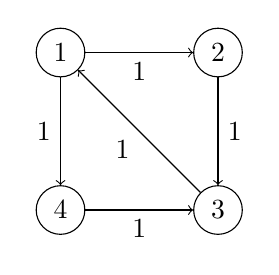
\begin{tikzpicture}[main/.style = {draw, circle}, node distance=2cm] 
\node[main] (1) {$1$}; 
\node[main] (2) [right of=1] {$2$}; 
\node[main] (3) [below of =2] {$3$}; 
\node[main] (4) [below of =1] {$4$}; 
\path (1) edge [->] node [below] {1} (2);
\path (2) edge [->] node [right] {1} (3);
\path (4) edge [->] node [below] {1} (3);
\path (1) edge [->] node [left] {1} (4);
\path (3) edge [->] node [below left] {1} (1);
\end{tikzpicture}
}}\]

In this graph there are only $5$ arcs and two integer-valued maximum circulations $\x'$ and $\x''$, each of value $3$. The circulation $\x'$ is obtained by sending one unit of flow on the cycle 1-2-3-1; the circulation $\x''$ is obtained by sending one unit of flow on the cycle 1-4-3-1.  This circulations and the remaining (residual flows) graphs, $G[V,\q-\x']$ and $G[V,\q-\x'']$ are:

\[
G[V,\x']=
\vcenter{\hbox{
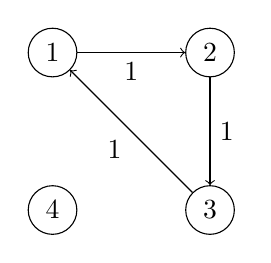
\begin{tikzpicture}[main/.style = {draw, circle}, node distance=2cm] 
\node[main] (1) {$1$}; 
\node[main] (2) [right of=1] {$2$}; 
\node[main] (3) [below of =2] {$3$}; 
\node[main] (4) [below of =1] {$4$}; 
\path (1) edge [->] node [below] {1} (2);
\path (2) edge [->] node [right] {1} (3);
%\path (4) edge [->] node [below] {1} (3);
%\path (1) edge [->] node [left] {1} (4);
\path (3) edge [->] node [below left] {1} (1);
\end{tikzpicture}
}}
\hspace{0.5in}
G[V,\q-\x']=
\vcenter{\hbox{
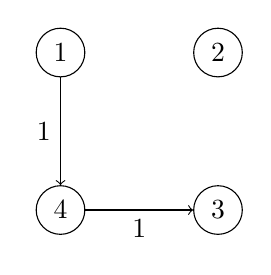
\begin{tikzpicture}[main/.style = {draw, circle}, node distance=2cm] 
\node[main] (1) {$1$}; 
\node[main] (2) [right of=1] {$2$}; 
\node[main] (3) [below of =2] {$3$}; 
\node[main] (4) [below of =1] {$4$}; 
%\path (1) edge [->] node [below] {1} (2);
%\path (2) edge [->] node [right] {1} (3);
\path (4) edge [->] node [below] {1} (3);
\path (1) edge [->] node [left] {1} (4);
%\path (3) edge [->] node [below left] {1} (1);
\end{tikzpicture}
}}
\]

\[
G[V,\x'']=
\vcenter{\hbox{
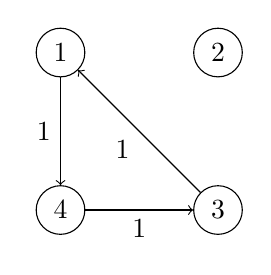
\begin{tikzpicture}[main/.style = {draw, circle}, node distance=2cm] 
\node[main] (1) {$1$}; 
\node[main] (2) [right of=1] {$2$}; 
\node[main] (3) [below of =2] {$3$}; 
\node[main] (4) [below of =1] {$4$}; 
%\path (1) edge [->] node [below] {1} (2);
%\path (2) edge [->] node [right] {1} (3);
\path (4) edge [->] node [below] {1} (3);
\path (1) edge [->] node [left] {1} (4);
\path (3) edge [->] node [below left] {1} (1);
\end{tikzpicture}
}}
\hspace{0.5in}
G[V,\q-\x'']=
\vcenter{\hbox{
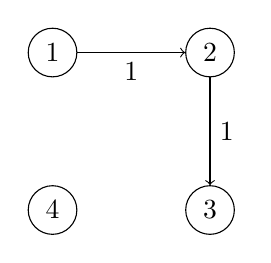
\begin{tikzpicture}[main/.style = {draw, circle}, node distance=2cm] 
\node[main] (1) {$1$}; 
\node[main] (2) [right of=1] {$2$}; 
\node[main] (3) [below of =2] {$3$}; 
\node[main] (4) [below of =1] {$4$}; 
\path (1) edge [->] node [below] {1} (2);
\path (2) edge [->] node [right] {1} (3);
%\path (4) edge [->] node [below] {1} (3);
%\path (1) edge [->] node [left] {1} (4);
%\path (3) edge [->] node [below left] {1} (1);
\end{tikzpicture}
}}
\]

Consider next the circulation $\x^* = (\x + \y)/2$ and the respective remaining graph after removing $\x$, $G[V,\q-\x ^*]$:
 
\[
G[V,\x^*]=
\vcenter{\hbox{
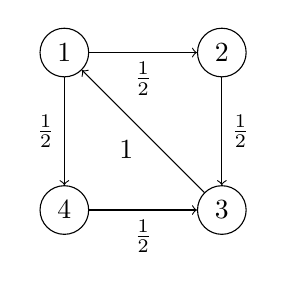
\begin{tikzpicture}[main/.style = {draw, circle}, node distance=2cm] 
\node[main] (1) {$1$}; 
\node[main] (2) [right of=1] {$2$}; 
\node[main] (3) [below of =2] {$3$}; 
\node[main] (4) [below of =1] {$4$}; 
\path (1) edge [->] node [below] {$\frac{1}{2}$} (2);
\path (2) edge [->] node [right]  {$\frac{1}{2}$} (3);
\path (4) edge [->] node [below] {$\frac{1}{2}$} (3);
\path (1) edge [->] node [left] {$\frac{1}{2}$} (4);
\path (3) edge [->] node [below left] {1} (1);
\end{tikzpicture}
}}
\hspace{0.5in}
G[V,\q- \x ^*]=
\vcenter{\hbox{
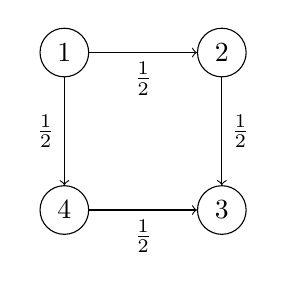
\begin{tikzpicture}[main/.style = {draw, circle}, node distance=2cm] 
\node[main] (1) {$1$}; 
\node[main] (2) [right of=1] {$2$}; 
\node[main] (3) [below of =2] {$3$}; 
\node[main] (4) [below of =1] {$4$}; 
\path (1) edge [->] node [below] {$\frac{1}{2}$} (2);
\path (2) edge [->] node [right]  {$\frac{1}{2}$} (3);
\path (4) edge [->] node [below] {$\frac{1}{2}$} (3);
\path (1) edge [->] node [left] {$\frac{1}{2}$} (4);
%\path (3) edge [->] node [below left] {1} (1);
\end{tikzpicture}
}}
\]

Note that the graph $G[V,\q- \x ^*]$ is acyclic, and therefore the set of arcs $A(\q- \x ^*)$ form an acylic graph. That follows since $\x ^*$ is a maximal circulation.  Note, however, that whereas the number of arcs in $A(\q-\x')$ is $2$ and the number of arcs in $A(\q-\x'')$ is $2$, the number of arcs in $A(\q-\x ^*)$ is $4$ and hence strictly greater than the number of arcs in the acyclic graph induced by the integer valued circulations. Following Lemma \ref{lem:strong-max}, $A(\q-\x^*)=A(\q-\x') \cup A(\q-\x'')$. Finally, by adding the transitive closure arcs to $A(\q- \x ^*)$, we get the strong partial order $A^{SP}$.  

\[
A(\q-\x ^*)=
\vcenter{\hbox{
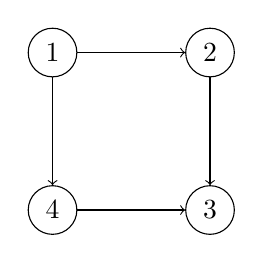
\begin{tikzpicture}[main/.style = {draw, circle}, node distance=2cm] 
\node[main] (1) {$1$}; 
\node[main] (2) [right of=1] {$2$}; 
\node[main] (3) [below of =2] {$3$}; 
\node[main] (4) [below of =1] {$4$}; 
\path (1) edge [->] node [below] {} (2);
\path (2) edge [->] node [right]  {} (3);
\path (4) edge [->] node [below] {} (3);
\path (1) edge [->] node [left] {} (4);
%\path (3) edge [->] node [below left] {1} (1);
\end{tikzpicture}
}}
\hspace{0.5in}
A^{SP}(\q)=
\vcenter{\hbox{
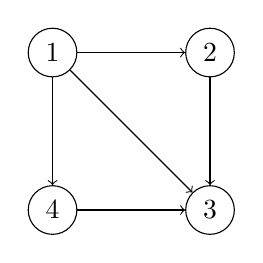
\begin{tikzpicture}[main/.style = {draw, circle}, node distance=2cm] 
\node[main] (1) {$1$}; 
\node[main] (2) [right of=1] {$2$}; 
\node[main] (3) [below of =2] {$3$}; 
\node[main] (4) [below of =1] {$4$}; 
\path (1) edge [->] node [below] {} (2);
\path (2) edge [->] node [right]  {} (3);
\path (4) edge [->] node [below] {} (3);
\path (1) edge [->] node [left] {} (4);
\path (1) edge [->] node [below left] {} (3);
\end{tikzpicture}
}}
\]



% \subsection{Three Methods for Constructing Consistent Rankings}\label{sec-rankings}
% \DO{Take out}
% \jnote{I am in favor of keeping some material on rankings.   We can point out that our focus is on partial orders, and one can derive complete rankings or weak rankings from partial orders. There are often exponentially many complete rankings consistent with a partial order.  One can also choose weak ranking where ties are permitted.  One natural choice of a weak ranking is where rank(i) is the length of the longest path to node i.}
% \NA{I cut the discussion of rankings down and moved it to the end of \ref{sec:strong-max-circulations} (right before the illustrative example). I am also fine with adding more to it or bringing it back to its own subsection.}





% \NA{The following two paragraphs were cut out of the definitions section:}
% \noindent \textbf{Rankings and ranks}. A {\em ranking} $r()$ is a mapping from the set of alternatives to the set of \emph{ranks}, represented by integers in $[1,n]$. Let $\r$ be a vector such that $r_i=r(i)$. A ranking is said to be {\em full} or {\em strict} if no ties are permitted; that is, each alternative is assigned a distinct rank.  A ranking in which ties are permitted is said to be {\em weak}. We define the rank of $1$ to be the most favorable (or best) rank. A vote $(i,j)$ is a voter's statement that the rank of $i$ should be strictly better than the rank of $j$; that is, the voter is saying that $r(i)$ should be strictly better than $r(j)$, or $r(i) < r(j)$. In general, we use the terminology ``better'' and ``worse'' in order to describe the ranks of alternatives as opposed to ``higher'' or ``lower.'' This alleviates the potential confusion with alternative approaches, e.g., \citet{hochbaum_methodologies_2006}, in which alternatives receive \emph{scores} and higher scores are better than lower scores.

% Suppose that $G=(V,A)$ is an acyclic graph.  A ranking is said to be {\em consistent} with the arc set $A$ if for every arc $(i, j) \in A$, $r(i) < r(j)$. Each topological ordering of an acyclic graph is  a consistent full ranking in which the rank of a node is its node label. There may also be weak rankings that are consistent. A \emph{minimum consistent ranking} is the consistent ranking for which each alternative receives its best possible rank.  A minimum consistent ranking can be determined in $O(m+n)$ time using a variant of the topological sort algorithm (see Subsection \ref{sec-rankings})

% --






% Recall that a ranking is weak or strict according as ties are or are not permitted.  
% Recall also that a ranking is consistent with the partial order induced by an acyclic graph $G=(V,A)$ if for every arc $(i, j) \in A$, $r(i) < r(j)$. 
% % That is, the  more-preferred alternatives receive lower integer value ranks than less-preferred alternatives. 

% % In this section we briefly describe methods for constructing consistent rankings from $A^{SP}$.

% %That is, if $i$ is preferred to $j$, $i\succ j$, then the numerical rank of $i$ must be \textit{less} than the rank of $j$, $r(i)<r(j)$, in any consistent ranking. This differs from methods in which alternatives receive scores, with higher scores being better. 

% The following are three alternative methods for constructing a consistent ranking for $A^{SP}$.

% \begin{enumerate}
%     \item {\bf Topological order.}  The topological order labels form a strong ranking in the sense that each alternative is assigned one distinct label/rank from $\{1,2,\ldots , n\}$.  
% %The topological order labeling is not unique.  If there are ties for the next nodes to be labeled, these ties are broken arbitrarily. In that sense the topological order is not an equitable method of assigning ranks.  
%     As described earlier, a topological order is any strict ranking that is consistent with $A^{SP}$.   The time it takes to find a topological order is $O(m+n)$. In general, there may be many distinct topological orders, perhaps exponentially many.
%     \item {\bf Minimum consistent ranking.}  A natural ranking is to assign each alternative its most favorable rank that is consistent with $A^{SP}$. One can obtain the minimum consistent ranking by modifying the algorithm for obtaining a topological order as follows: whenever the algorithm has a choice for the next node to label, all candidate next-rank nodes get the next label.
%     \item {\bf Maximum consistent ranking.}  This approach is the mirror image of the application of most favorable ranking.  The algorithm first computes the maximum (i.e., worst) rank obtained in the minimum consistent ranking.  Suppose that this rank is $k$.   Then the ranks of nodes are assigned in reverse order:  Nodes that have no successors (are not preferred to any other alternative) are assigned a rank of $k$.  Once these are removed, every node that does not have successors is assigned the rank of $k-1$, etc.  
%     %In any acyclic graph there must be at least one node with no successors, so the process will terminate once all the nodes are labels.  Note that if the most favorable rank is $r$, then $k-r$ is also the length of the longest path in the acyclic graph.
%     This procedure will always result in the most favorable ranking being a rank of 1.
% \end{enumerate}

% In Section \ref{sec:dual-optimal-rankings} we further discuss rankings that are consistent with the dual linear program.

\section{%A Very Efficient Algorithm for 
Computing a Strong Circulation with One Maximum Circulation Flow }
\label{sec:certif}

Algorithm 1, described
in Section \ref{sec:strong-max-circ}, computes the acyclic graph $A^*$, which in turn can be used to construct a strong maximum circulation and a strong partial order.
Algorithm 1 requires solving at most $m+1$ maximum circulation problems.  In this section, we introduce the  \emph{perturbation algorithm}, which determines $A^*$ by solving a single minimum cost network flow (MCNF) problem.  Specifically, the preturbation algorithm returns a strong maximum circulation, which is then used to find $A^*$ by removing the arcs at capacity.

The perturbation algorithm relies on the optimality conditions that are shown to characterize strong maximum circulations---the {\emph{strong complementary slackness conditions}, as defined in Subsection  \ref{sec:strong}. The formulation of the associated MCNF problem and the perturbation algorithm are subsequently given in Subsection \ref{sec:more-efficient}.
%we demonstrated how cycle removal methods can be used to obtain $A^*$, which in turn induces the strong partial order.  We  showed how to obtain this order by solving at most $m+1$ maximum circulation problems. In this section, we show how to determine $A^*$ by solving a single minimum cost network flow (MCNF) problem.  The solution to the MCNF problem is transformed into a strong maximum circulation.  After removing the arcs at capacity, what remains is $A^*$. 

\subsection{Strong (Rather than Strict) Complementary Slackness}
\label{sec:strong}
We define here the ``strong complementary slackness" conditions that are proved to characterise strong maximum circulations.
%We begin with optimality conditions based on the formulation of the maximum circulation problem that we refer to as ``strong complementary slackness.''
These conditions are more restrictive than the usual complementary slackness conditions, but less restrictive than the conditions that are known as strict complementary slackness.  We will subsequently show that the strong maximum circulation derived from the MCNF solution satisfies strong complementary slackness.


Among all optimal solutions for the maximum circulation problem \ref{eqn:max-circ}, we want a strong maximum circulation; that is, we want a maximum circulation with as many arcs as possible with flow less than than their capacity.  Suppose that we were given a circulation $\x'$.  One can identify that $\x'$ is maximum using a form of LP duality such as the complementary slackness conditions. It is shown next that one can identify that $\x'$ is strong if it satisfies the ``strong complementary slackness conditions.''


The dual of the maximum circulation problem (\ref{eqn:max-circ}) is:


\begin{align}
    \label{eq:dual-program}
      \min & \sum_{(i,j)\in A} q_{ij}z_{ij} \\
     \text{subject to } & y_i -y_j +z_{ij} \ge 1 \,\, \forall (i,j)\in A \nonumber\\
     &z_{ij} \ge 0 \,\, \forall (i,j)\in A. \nonumber
\end{align}


Suppose that $\x'$ is a feasible circulation for (1), and  that $(\y', \z')$ is feasible for (\ref{eq:dual-program)}.  We will express the strong optimality conditions based entirely on the vectors $\x'$ and $\y'$.  We may do so without loss of generality because we assume that for all $(i,j) \in A$, $z'_{ij}=\max \{ y'_j-y'_i +1, 0\}$.  These conditions are satisfied by any optimal solution to (\ref{eq:dual-program}).


We use the notation $\c$ for the vector of cost coefficients in a MCNF problem, which for the primal maximum circulation problem (\ref{eqn:max-circ}) satisfy $c_{ij} = 1$ for all $(i, j) \in A$.   We say that $\x'$ and $\y'$ satisfy \emph{strong complementary slackness} for the MCNF problem if the following is true:

\begin{enumerate}
\item  For each $(i,j) \in A$, if $x'_{ij} = 0$, then $c_{ij} - y'_i + y'_j  \le  0$.
\item  For each $(i,j) \in A$, if $0 < x'_{ij} < q_{ij}$, then $c_{ij} - y'_i + y'_j  =  0$.
 \item  For each $(i,j) \in A$, if $x'_{ij} = q_{ij}$, then $c_{ij} - y'_i + y'_j  >  0$.

\end{enumerate}

The above conditions are more restrictive than the standard complementary slackness conditions because of (3).    The usual complementary slackness condition is: ``if $x'_{ij} = q_{ij}$, then $c_{ij} - y'_i + y'_j  \ge  0$".  The above conditions are also less restrictive than {\em strict} complementary slackness conditions, which require,  in addition to (2) and (3), to replace (1) by:  ``For each $(i,j) \in A$, if $x'_{ij} = 0$, then $c_{ij} - y'_i + y'_j  <  0$". 

If $\x'$ and $\y'$ satisfy strong complementary slackness, then $\y'$  ``certifies'' that $\x'$ is a strong maximum circulation, as stated in the following lemma.

\begin{theorem} \label{lem:comp-slack-strong}
  Suppose that $\x'$ is a feasible circulation for (\ref{eqn:max-circ}), and that $\y'$ is feasible for (\ref{eq:dual-program})---i.e., the dual of (\ref{eqn:max-circ}).  If $\x'$ and $\y'$ satisfy strong complementary slackness, then $\x'$ is a strong maximum circulation. 
\end{theorem}
\begin{proof}
    Assume that $\x'$ and $\y'$ satisfy strong complementary slackness. Then they also satisfy complementary slackness, and are thus optimal for the respective primal (\ref{eqn:max-circ}) and dual (\ref{eq:dual-program}) problems. Therefore $\x'$ must be a maximum circulation and  $\y'$ is a dual optimal solution.
    To prove that $\x'$ is a strong maximum circulation, 
    we show next that for any other maximum circulation  $\x''$, if $x'_{ij}=q_{ij}$ for any arc $(i,j) \in A$, then $x''_{ij}=q_{ij}$.

 % Suppose now that $\x''$ is any other maximum circulation. 
   % We now claim that if $x'_{ij}=q_{ij}$ for any arc $(i,j) \in A$, then $x''_{ij}=q_{ij}$.  If this claim is true, then $\x'$ is a strong maximum circulation.  We see that the claim is true as follows. 
By the strong complementary slackness satisfied by
$\x'$ and $\y'$: if $x'_{ij}=q_{ij}$, then $c_{ij} - y'_i + y'_j  >  0$.  Since $\x''$ is a maximum circulation and  $\y'$ is a dual optimal solution, it follows that  $\x''$ and $\y'$ satisfy complementary slackness.   Therefore $c_{ij} - y'_i + y'_j  >  0$, implies that $x''_{ij}=q_{ij}$.   
\end{proof}

\subsection {The ``Perturbation" Algorithm}
\label{sec:more-efficient}
We present here the ``Perturbation" algorithm that
finds a strong maximum circulation $\x^*$ as well as the set $A^*$ and the induced strong partial order $A^{SP}$ by solving a single maximum (or minimum) cost flow problem derived from a ``perturbation" of the maximum circulation problem.   That solution also produces a dual vector $\y^*$ such that $\x^*$ and $\y^*$ satisfy strong complementary slackness.

The perturbation algorithm relies on solving the following maximum utility (negative cost) flow problem with two sets of decision variables $\w , \v \in \mathbb{R}^m$.  Recall that $m=|A|=|A(\q)|$, the number of arcs in the vote graph $G=(V,A)$.  Our network flow formulation (\ref{eqn:max_xy}) is defined on a graph $G=(V,A^{(2)})$ where $A^{(2)}$ contains 2 copies of each arc $(i,j) \in A$.  The flow in the first copy of $(i, j)$ will be denoted as $w_{ij}$ with capacity upper bound $q_{ij} - \epsilon$, and the flow in the second copy of $(i,j)$ will be denoted as $v_{ij}$ with capacity upper bound $\epsilon$.  If $q_{ij}$ is integral for all arcs $(i,j) \in A$, then we can choose $\epsilon = 1/(m+1)$.  Otherwise, we can choose $\epsilon = 1/( (m+1)\cdot LCD)$, where LCD is the least common denominator of the values in the vector $q$.

We let $c_{ij} = 1$ for all arcs $(i,j) \in A$.  

 \begin{align}
    \label{eqn:max_xy}
      \max \,\,\,\,\ & f(\w, \v) =   \sum_{(i,j)\in A} c_{ij} (w_{ij}+v_{ij})
      -\frac{1}{m+1} \sum_{(i,j)\in A} v_{ij}\\
      \text{subject to } & \sum_{j: (i,j) \in A} (w_{ij}+v_{ij})-\sum_{j:  (j,i) \in A}( w_{ji}+v_{ji})=0  \,\,\ \forall i\in V, \nonumber\\     
 %     \nabla w_i \nonumber
 %     + \nabla v_i = 0 \,\,\, \text{ for }i \in V \\
     & 0\leq w_{ij} \leq q_{ij} - \epsilon \nonumber
     \,\,\, \text{ for }(i,j) \in A, \\
     & 0\leq v_{ij} \leq \epsilon \nonumber
     \,\,\,\, \text{ for }(i,j) \in A. 
\end{align}

\medskip

We note that model \ref{eqn:max_xy} is a maximum cost flow problem. %\DO{I think it is a maximum circulation problem?}  \jnote{Answered earlier.} 
It can be converted to a minimum cost flow problem by replacing the objective function by its negative.

The perturbation algorithm consists of first finding an optimal solution $(\w', \v')$ for problem (\ref{eqn:max_xy}), and then finding an optimal solution $(\y', \z')$ for the dual of (\ref{eqn:max_xy}).  The complexity of finding an optimal solution to MCNF, using the successive approximation algorithm of \cite{goldberg_solving_1987}, is $O(nm \log (n^2/m) \log(nC))$, where $n=|V|$ $m=|A|$ and $C=\max _{(i,j)\in A} |c_{ij}|$.  Here we scale the objective function  
by $m+1$ so all coefficients are integer, and $C=m+1$. Observing that $m=O(n^2)$ the complexity of solving (\ref{eqn:max_xy}) is $O(nm \log(n^2/m)\log n )$ -- the same complexity as that of solving one maximum circulation problem.
To derive the optimal dual solution, the standard procedure is to construct a graph where the arcs are all the residual arcs with respect to the optimal flow, with their respective costs, and to add a source node with arcs of length $0$ to all nodes in the graph.  In this constructed graph the length of the shortest paths from the source node, correspond to the optimal dual values.  Hence, the optimal dual solution $\y'$ can be obtained in $O(mn)$ time, using, e.g., the Bellman-Ford algorithm. This time to determine the optimal dual solution is dominated by the run time required to find the optimal flow.

% \DO{Jim: How do you get the dual in $O(m)$?} 
% \jnote{For a basic feasible solution, the dual variable for node j is the length of the path from node j to the root node in the optimal spanning tree.}
% \DO{But I am not convinced that the algorithm of successive approximation gives a basic solution. And why should we bother anyway, as the single source shortest paths is $O(mn)$ which is good enough.}

The perturbation algorithm outputs $\x' = \w' + \v'$.  We show next that $\x'$ is a strong maximum circulation and that $(\x', \y')$ satisfies strong complementary slackness for the maximum circulation problem.

\begin{lemma}
\label{equivalent}
Let $(\w', \v')$ be an optimal basic solution for the maximum cost network flow problem (\ref{eqn:max_xy}) and $(\y',\z')$ optimal for the dual linear program.   Then $\x' = \w' + \v'$ is a strong maximum circulation and $A'= \{(i, j): v'_{ij} = 0\}$ satisfies $A' = A^*$.  
Moreover, $\x'$ and $\y'$ satisfy strong complementary slackness for the maximum circulation problem  (\ref{eqn:max-circ}). 
%\DO{It is enough to show the strong complementary slackness since we proved in Lemma \ref{lem:comp-slack-strong} that this implies the rest.} \jnote{Yes.}
\end{lemma}
\begin{proof}

We first consider a solution to (\ref{eqn:max_xy}) that is derived from a strong maximum circulation.  Let $\x ^*$ be the strong maximum circulation calculated by averaging the flows from Algorithm 1.  Let
$A^* = A(q - \x^*)$ denote the arcs whose flow are not at capacity in $\x ^*$.  By Lemma \ref{lem:strong-max}, $A^*$ is the set of strong arcs. Let $K = |A^*|$.  Thus $K < m$.  Note that $\x ^*$ is obtained as the average of $K$ basic flows.  Assuming that all capacities are integral, for each arc $(i, j) \in A^*$, $x^*_{ij} \le q_{ij} - \frac{1}{K} < q_{ij} - \epsilon$.

Let $(\w^*, \v^*)$ be derived from $\x ^*$  as follows.  If  $x^*_{ij}< q_{ij} - \epsilon$, then $w^*_{ij} = x^*_{ij}$ and $v^*_{ij} = 0$.  If  $x^*_{ij}= q_{ij}$, then $w^*_{ij} = x^*_{ij} - \epsilon$ and $v^*_{ij} = \epsilon$.   Note that $(\w^*, \v^*)$ is feasible for the maximum cost flow problem (\ref{eqn:max_xy}).
Let $\eta^*$ be the optimal objective for the maximum circulation problem.   Then $f(\w^*, \v^*) = \eta^* - \frac{(m-K) \epsilon}{m+1} > \eta^* - \epsilon  $. 

We next establish the optimality of $\x'$ for  (\ref{eqn:max-circ}).
Note that $f(\w', \v') \ge f(\w^*, \v^*) > \eta^* - \epsilon$.  Therefore, $\c \cdot \x' > \eta^* - \epsilon$.   Since $(\w', \v')$ is a basic solution, it follows that all flows are integral multiples of $1/\epsilon$, and thus $\c \cdot \x' \ge \eta^* $, implying that $\x'$ is optimal for the maximum circulation problem.

We next show that $A' = A^*$, and thus, according to Corollary \ref{lem:strong-max}, $\x'$ is a strong maximum circulation.  Since $f(\w', \v') = \eta^* - \frac{(m-|A'|)\epsilon}{m+1} \ge 
f(\w^*, \v^*) = \eta^* - \frac{(m - |A^*|)\epsilon}{m+1}$, it follows that $|A'| \ge |A^*|$.  And because $\x'$ is a maximum circulation and $\x^*$ is a strong maximum circulation, it follows that $A' \subseteq A^*$.  We conclude that $A' = A^*$, and therefore $\x'$ is a strong maximum circulation.

Because $A' = A^*$, it follows that $f(\w^*, \v^*) = f(\w', \v')$.  Therefore, $(\w^*, \v^*)$ is optimal for (\ref{eqn:max_xy}).


% Let $A^*$ be set of arcs whose flow is not at capacity in at least one maximum circulation.  Let $K = |A^*|$.  Thus the flow in each of the $m - K $ arcs in $A\backslash A^*$ is at capacity in every maximum circulation.   Let $z^*$ denote the optimal objective  value for (\ref{eqn:max-circ}).   Let $\x ^*$ be a strong maximum circulation calculated by averaging the flows from Algorithm 1.  That is, $\x ^*$ is the average of  $K$ different optimal basic solutions, where $K \le m$.  Accordingly, $x^*_{ij} <  q_{ij} - \epsilon$ for all $(i, j) \in A^*$.  Let $(\w^*, \v^*)$ be defined as follows.  If $(i, j) \in A^*$, then $w^*_{ij} = x^*_{ij}$ and $y^*_{ij} =0$.   

% We will show that if $\x'$ is not optimal for (\ref{eqn:max-circ}), then $f(\w', \y') < f(\w^*, \y^*) $, which contradicts the optimality of $(\w', \y')$ for (\ref{eqn:max_xy}).  
% Suppose now that $\x'$ is not optimal for   (\ref{eqn:max-circ}).  Because all flows are multiples of $\epsilon$, it follows that $\sum_{(i,j)\in A}x'_{ij} \le z^*-\epsilon$, in which case $f(\w', \y')  \le z^*-\epsilon$.

% We note that $(\w^*, \y^*)$ is feasible for (\ref{eqn:max_xy}).  Moreover its objective value is 

% $$f(\w^*, \y^*) = z^* - \frac{\epsilon(m - K)}{m} > z^*-\epsilon \ge f(\w', \y').$$  

% This contradiction shows that $x'$ is optimal for  (\ref{eqn:max-circ}).  

% We now claim that $(\w^*, \v^*)$ is optimal for (\ref{eqn:max_xy}).   To see why, note that 
% $f(\w^*, \v^*) =  z^* - \frac{\epsilon(m - K)}{m}$.  Since $x'$ is optimal for (\ref{eqn:max-circ}), it follows that each arc $(i,j) \in A\backslash A^*$ has $x'_{ij} = q_{ij}$, and thus $f(\w^*, \v^*) \le  z^* - \frac{\epsilon(m - K)}{m}$.  This establishes the claim.

% We now claim that $\x'$ is a strong maximum circulation.   This follows from the fact that $f(\w', \v') = f(\w^*, \v^*)$, and thus the only arcs at capacity for $\x'$ are the arcs of $A\backslash A^*$.  

We next show that $\x^*$ and $\y'$ satisfy strong complementary slackness conditions for (\ref{eqn:max-circ}).  We see why as follows.  Because $(\w^*, \v^*)$ is optimal for (\ref{eqn:max_xy}),  $(\w^*, \v^*)$ and $\y'$ satisfy complementary slackness conditions for (\ref{eqn:max_xy}).  Therefore,  the following is true: 
 
\begin{enumerate}
\item  For each $(i,j) \in A$, if $x^*_{ij} = 0$, then $w^*_{ij} = 0$, and $c_{ij} - y'_i + y'_j  \le  0$.
\item  For each $(i,j) \in A$, if $0 < x^*_{ij} < q_{ij}$, then $0 < w^*_{ij} < q_{ij} - \epsilon$, and  $c_{ij} - y'_i + y'_j  =  0$.
\item  For each $(i,j) \in A$, if $x^*_{ij} = q_{ij}$, then $v^*_{ij} = \epsilon$, and $(c_{ij} - \frac{1}{m+1}) - y'_i + y'_j  \ge  0$, which implies that $c_{ij} - y'_i + y'_j  >  0$.
 \end{enumerate} 
 
 Thus, $\x^*$ and $\y'$ satisfy strong complementary slackness.

Finally, we show that $\x'$ and $\y'$ satisfy strong complementary slackness, which will complete the proof of this lemma:  Clearly, $\x'$ and $\y'$ satisfy the first and third conditions of strong complementary slackness.   As for the second condition, 

$$ \text{If } 0 < x'_{ij} < q_{ij}, \text{ then } 0 < x^*_{ij} < q_{ij} - \epsilon, \text{ and } c_{ij} - y'_i + y'_j  =  0.$$
\end{proof}


% \NA{Reviewer 4 noted that we should have $y_i'$ and $y_j'$ instead of $y_i$ and $y_j$ on this page. I'm a bit unsure on where they are referring to.}
% \SG{All of the $y_i$ and $y_j$ in the strong complementary slackness claim should be $y'_i$ and $y'_j$, I believe. I've made the edits in text.}

% \section{Preprocessing by Eliminating 2-Cycles First}\label{sec:2-cycle}
% \DO{Take this out}
% \jnote{This section may distract from the rest of the paper.  It's fine with me if we remove it.} 
% \NA{That's fine with me. We should just point to the possibility in the conclusion.}
% To this point, we have introduced the concept of a strong maximum circulation, shown the uniqueness of the strong partial order, demonstrated how to construct consistent ranks from the strong partial order, and proposed an efficient algorithm for computing the strong partial order. A natural question is whether there exists an alternative efficiently computable cycle-elimination method that eliminates fewer votes and also produces a unique solution. In this section, we describe a simple 2-phase variant of maximum cycle elimination. In the first phase, cycles of length 2 are eliminated. In the second phase, the algorithm produces a strong maximum circulation in the remaining vote graph.  This approach frequently eliminates fewer votes than a strong maximum circulation.

% %Although minimum-maximal-cycle-based elimination methods are consistent with the spirit of Kemeny's method by eliminating the minimum number of votes, they also face many of the drawbacks of Kememy's method. Maximum cycle elimination methods overcome these problems at the cost of eliminating more votes. In this subsection, we describe a variant of maximum cycle elimination that frequently eliminates fewer votes than the strong maximum circulation. 


% %This is an example of a broader class of cycle cancelling methods in which the vote graph is pre-processed by initially eliminating smaller-size cycles and then applying the strong maximum circulation to the revised vote graph. 

% The graph in Figure \ref{fig:2cycle-a} illustrates how cancelling 2-cycles first can lead to a residual acyclic graph with many additional arcs. 
% %A potential advantage of first cancelling 2-cycles can be seen by considering the acyclic preference graph in Figure \ref{fig:2cycle-a}. 
% The preferences in the example are a complete order in which $1\succ 2 \succ \ldots \succ n$. Now consider adding one vote for $n$ preferred to $1$ and a second vote for $1$ preferred to $n$, resulting in the (cyclic) preference graph in \ref{fig:2cycle-b}. Removing the 2-cycle leads the original complete order to be returned. In contrast, the unique strong maximum circulation for \ref{fig:2cycle-b} consists of the cycle 1-2-\ldots-$n$-1. After removing this cycle, the resulting strong partial order is given by  \ref{fig:2cycle-c}. That is, the addition of the 1-$n$-1 cycle resulted in the removal of a large number of votes, and only left the vote for $1$ over $n$. 


% %Let $\x_{(2)}$ represent a circulation consisting of the maximum number of 2-cycles and let $\x^*(\q-\x_{(2)})$ be a strong maximum circulation defined with respect to $G[V, \q - \x_{(2)}]$,

% %Whether this is a desirable characteristics of strong maximum cycle elimination is unclear. On the one hand, it is not unreasonable that adding a new vote for the worst-ranked alternative over the best-ranked alternative would improve the ranking of the former and hurt the ranking of the latter. On the other hand, pre-processing the vote graph by removing 2-cycles prior to computing the strong maximum circulation leads fewer votes to be eliminated and thus counteracts some of the conservatism inherent to the proposed approach. Specifically, by defining the strong partial order from the net graph instead of the original vote graph, the strong partial order is made to be insensitive to the addition of 2-cycles. To see this, note that the pre-processing step applied to \ref{fig:2cycle-b} would result in the removal of the 1-n-1 cycle, and the resulting partial order would be given by the original acyclic preference graph, Figure \ref{fig:2cycle-a}. 

% %\JO{I would omit the above paragraph.  I don't think we have a lot to say about whether eliminating 2-cycles first is a good idea.}\NA{That's fine with me.}\\

% % Figure environment removed

% Eliminating 2-cycles first and then eliminating a strong maximum circulation also has the desirable property of satisfying the Condorcet criterion, which we describe next.  An alternative $i$ is called a \textit{Condorcet winner} if  $q_{ij}>q_{ji}$ for all $j\neq i$.  An aggregation method is said to satisfy the \textit{Condorcet criterion} if the aggregation method is guaranteed to produce a partial order in which a Condorcet winner (if one exists) is  preferred to all other alternatives. We observe that a strong partial order does not necessarily satisfy the Condorcet criterion.\footnote{Consider three voters with preference $1\succ2\succ3$ and two voters with preferences $2\succ3\succ1$ so that the vote graph is given by $q_{12}=3$, $q_{13}=3$, $q_{21}=2$, $q_{23}=5$, $q_{31}=2$, and $q_{32}=0$. Alternative $1$ is a Condorcet winner. However the unique maximum circulation consists of pushing one unit of flow on the cycle 1-2-3-1, two units of flow on the cycle 1-2-1, and one unit of flow on the 1-3-1 cycle. This results in $A^{SP}=\{(1,3),(2,3)\}$.}  
% However, if all 2-cycles are removed first, then the resulting strong partial order does satisfy the Condorcet criterion.

% % inducing a partial order in which a Condorcet winner is undominated. We say that an aggregation method satisfies the \textit{Condorcet criterion} if when $q_{ij}>q_{ji}$ for all $j\neq i$, $i$ is the unique winner (the \textit{Condorcet Winner}). 

% % Note that 

% \begin{lemma}
%  If $G[V, \q]$ be a vote graph and let $G[V, \q']$ be obtained by removing all 2-cycles, then the strong partial order induced by $G[V, \q']$ satisfies the Condorcet criterion.
% \end{lemma}
% \begin{proof}
%     Let $i$ be a Condorcet winner: $q_{ij}>q_{ji}$ for all $j\neq i$. Let $q'_{ij}$ represent votes for $i$ over $j$ after removing pairwise cycles. Observe that $q'_{ij}>0$ and $q'_{ji}=0$ for all $j\neq i$. 
    
%     Because there are no arcs going into $i$ in $\q'$, there can be no other cycles that cancel any remaining arcs leaving from $i$. Therefore $(i,j)\in A^{TC}(\q' - \x^*)$, $\forall j\neq i$.
% \end{proof}

% It follows immediately that first removing 2-cycles also guarantees that a Condorcet Winner is the unique winner in any consistent ranking.

\section{Dual Optimal Rankings and the Hochbaum-Levin Model}\label{sec:HL}
We now discuss rankings that are consistent with the dual linear program of the maximum circulation problem. We begin by introducing the separation-deviation model of \cite{hochbaum_methodologies_2006}, which links the Kemeny model to maximum cycle removal methods, and we show that the convex relaxation of Kemeny's model is the dual of the maximum circulation problem (but not the strong maximum circulation problem). %In Subsection \ref{sec:dual-optimal-rankings}, we show that all solutions to the convex relaxation of Kemeny's model are consistent with the strong partial order, but the converse is not true.  That is, a solution that is consistent with the strong partial order is not necessarily consistent with the convex relaxation of Kemeny's model. 

The Hochbaum and Levin model, henceforth called the HL model, determines a score for each alternative so that the vector of scores minimizes a loss function.  The voting system permitted in the HL model is more general than the preference votes studied here: Each voter may provide a score for each alternative, as well as a pairwise preference, that is expressed with intensity of preference for each pair of alternatives (e.g., the differences in ranks among pairs of alternatives in a voter's ranked list).

Given the more general voting system in the HL model, we will refer to voters in this section as {\em reviewers}.  
% A reviewer $r$ may submit a score  for some or all of the alternatives, and may submit pairwise preferences that correspond to the intensity of the (additive) difference in scores. 
For each alternative $i$, each reviewer $r$ can submit a score denoted as $s^r_i$.  For each pair of alternatives $i$ and $j$, reviewer $r$ can submit a preference of $i$ over $j$ with intensity $p^r_{ij}$. 


%In the language of the HL model, a vote in our paper is expressed as $p^r_{ij} \ge 1$ meaning that the score of $i$ is strictly higher than that of $j$ by at least one unit.

The decision variables for the HL model are the components of the vector $\y$, where $y(i)$ is the score of alternative $i$; the higher the score, the more preferred the alternative. 


For each reviewer $r$ and alternative $i$, there is a loss $g_i^r(y(i) - s^v_i)$, which is a function of the {\em deviation} of the final score from the score that reviewer $r$ provides for alternative $i$.  For each reviewer $r$ and for each pair $i,j$ of alternatives, there is a loss {\em separation} function $f^r_{i,j}(p^r_{ij} - (y(i)- y(j)))$, which is a function of the solution's difference in scores as compared to the intensity of the preference of reviewer $r$ for this pair $i,j$.  Both the separation and deviation functions take the value $0$ for zero valued arguments. 

As before, we let $V$ be the set of alternatives, and $A$ the set of pairs $(i,j)$ where at least one reviewer expresses a preference of $i$ over $j$.
We assume that $g^r_i(0) = 0$ for all $i \in V$ and $r \in R$.  We also assume that $f^r_{ij}(0) = 0$ for all $i,j \in V$ and $r \in R$.  Accordingly, if the voter's score or preference is identical to the solution's, then the loss penalty is zero. The HL model is to determine a ranking that minimizes the total deviation and separation loss for all voters.  

 Let $R_{ij}$ be the set of reviewers that express a preference of $i$ over $j$.  Let $R_i$ be the set of reviewers that assigned a score to alternative $i$.  Recall that $q_{ij}=|R_{ij}|$ is the number of votes expressing a preference of $i$ over $j$. The variables
$y(i)$ can take (continuous) values in an interval, or they can be restricted to take integer values in a given range.

The overall model is to minimize the aggregate loss function:
$$({\rm HL})\ \ \ \min Loss(\y)=\sum _{i\in V} \sum _{r\in R_i}g_i^r(y(i)-s_i^r) + \sum _{(i,j)\in A} \sum _{r\in R_{ij}} f_{ij}^r(y(i)-y(j)-p^r_{ij}).$$

Hochbaum and Levin showed how to solve the optimization problem (HL) in polynomial time when the functions $g_i^r()$ and $f_{ij}^r()$  are convex. They  showed how to solve this convex problem in polynomial time for integer variables (and also for continuous variables). %\jnote{I clarified that the integer program is solvable in polynomial time for the convex case.} 
% \DO{Yes, that is correct.  For general convex functions the continuous solution is to be $\epsilon$-accurate, which means it is specified with finite accuracy on $\epsilon$ grid, and each variable value is at most $\epsilon$ distance away from the optimal value of the variable.  The value of $\epsilon$ is user specified and no digital computer can provide an optimal solution with $\epsilon =0$ to nonlinear non-quadratic convex optimization problems.  The running time is polynomial in $\log 1/\epsilon$.} 
This problem was shown to be a special case of the {\em convex dual of minimum cost network flow}, which is solved by the algorithm of \cite{AHO03} in $O(nm\log {\frac{n^2}{m}}\log nU )$, where $n$ is the number of alternatives $|V|$, $m$ is the number of different $f_{ij}$ functions, and $U$ is the range of the variables. For example, if the components of $\y$ are constrained to fall in the range $[-n,n]$, then $U = 2n$.  When the functions are non-convex, then the problem is NP-hard, see, e.g., \cite{GT2000}.  

The preference voting system considered here is a special case of that in HL in which $R_i = \emptyset$ for all $i\in V$, and where $p^r_{ij} = 1$ for all $r \in R_{ij} $. That is, whenever reviewer $r$ prefers alternative $i$ to alternative $j$ it is associated with an intensity of $1$ unit. In addition, all decision variables (scores) are required to be integer valued.
For each $r \in R_{ij}$, there is an associated loss in the objective function of $f_{ij}^r(y(i)-y(j)-1)$.

We observe that Kemeny's model can be represented as a special case of the HL model.  Let  $\delta^+(z)$ denote the function that takes the value $1$ when $z >0$ and zero otherwise. With this notation, 
% consider the separation function penalty $f_{ij}^r(y(i)-y(j)-p^r_{ij}) = \delta^+(y(j)-y(i)+1)$ that charges one unit for each 
% preference vote that is violated by the final ranking.
Kemeny's model can be expressed as a special case of the HL model as follows:

$$(\text{KEM}) \,\,\,\,\, \min  \sum _{(i,j)\in A}  q_{ij}\delta^+(y(j)-y(i)+1).$$


This objective function is non-convex, and there is no known efficient algorithm for solving it. Recall that finding an optimal solution to the Kemeny model is NP-hard.

Taking a convex relaxation of the objective in Kemeny's model, one obtains the following convex loss function for the resulting optimization problem: 

$$(\text{Relax-KEM}) \,\,\,\,\, \min  \sum _{(i,j)\in A}  q_{ij}\max\{(y(j)-y(i)+1), 0\}.$$
 
 \cite{gupte_finding_2011} created a model equivalent to Relax-KEM. where they referred to the loss function as the ``agony'' loss function.  They also showed that Relax-KEM is the dual of the problem that we refer to as the maximum circulation problem. This result is a special case of the fact that convex HL and the convex separation-deviation model is a convex cost dual network flow problem 
 \citep{hochbaum_methodologies_2006,hochbaum2001MRF}.  We provide their result as well as a more concise proof next.

 \begin{lemma}
 \label{lem:DualKEM}
 (Relax-KEM) is the equivalent to the dual of the maximum circulation problem (\ref{eqn:max-circ}).    
\end{lemma}
\begin{proof}   
The dual to the maximum circulation problem is LP (\ref{eq:dual-program}). Recall that any optimal solution $(\y, \z)$ to \ref{eq:dual-program} satisfies the following:   $z_{ij}=\max \{ y_j-y_i +1, 0\}$. Therefore, if $(\y, \z)$ is optimal for (\ref{eq:dual-program}), then
$y(i) = y_i$ minimizes (Relax-KEM).
 \end{proof}

The maximum circulation problem has the property that all cost coefficients are 1.  If the optimum vector of dual variables $\y'$ is calculated based on an optimal spanning tree solution (see for example, \cite{ahuja_network_1993}),  then $\y'$ is integral, and $|y'_i - y'_j| \le n-1$ for all $i,j \in V$.  By subtracting $1+\max\{y'_i : i \in V\}$ from all coefficients in $\y'$ one obtains an optimal dual solution in which all coefficients are in the range $ \{-n, ..., -1\}$.

% For this dual network flow problem, there is always an optimal solution $\y', \z'$, such that for all $i \in V$, $y'_i$ lie in any interval of length $n - 1$, e.g., in $ \{-n, ..., -1\}$,  and so that at least one $y'_i$ has its value equal to $-1$, and so that the values taken on by the vector $\y'$ are integers.

%\NA{Reviewer 4 says that it would be better to have a proof for the above paragraph.}
%\jnote{Dorit, do you think that the revised paragraph above can substitute for a proof?} \DO{I think it is good now.}
 
Consequently, the approach of the maximum circulation can be viewed as the dual of Kemeny's method's convex relaxation of the penalty minimization formulation (KEM). 


\section{Minimum Maximal Circulations} \label{sec:minmax}

%We now consider basing rankings on the removal of minimum maximal circulations rather than maximum circulations. That is, methods based on removing cycles with the fewest number of total votes rather than the most votes. We show that an approach based on minimum maximal circulations shares two of the same shortcomings of Kemeny's approach. First, the partial orders induced from two different minimum maximal circulations may conflict with one another. And second, finding even a single minimum maximal circulation is NP-complete.



A natural counterpart of Kemeny's method in our setting is to find a maximal circulation that removes a minimum number of votes. We refer to this problem as the {\em minimum maximal circulation problem}. While this problem does have the desirable property of having as many votes as possible included in the acyclic graph, it also comes with the following drawbacks, which are established next.
\begin{enumerate}
    \item {\bf Non-uniqueness}: There may be more than one minimum maximal circulation. Further, these minimum maximal circulations may induce conflicting partial orders. That is, there may be minimum maximal circulations $\x'$ and $\x''$ and a pair of alternatives $i$ and $j$ such that $(i,j) \in A^{TC}[V,\q - \x'] $ and $(j, i)\in A^{TC}[V,\q - \x'']$, as shown in Subsection \ref{sec:minimax-equitable}. 
    \item {\bf NP-hardness}: Finding a minimum maximal circulation is NP-hard, as shown in Subsection \ref{sec:minmaxNPhard}.
\end{enumerate}


\subsection{Minimum Maximal Circulations Can Induce Conflicting Partial Orders}\label{sec:minimax-equitable}

In this subsection, we show that there may be two different minimum maximal circulations that lead to conflicting partial orders. Cycle cancelling approaches based on minimum maximal circulations thus face similar normative challenges as Kemeny's method. Alternatives receive more or less favorable treatment depending on which set of votes is eliminated.

Consider the vote graph $G = (V, A)$, illustrated in the top panel of \autoref{fig:minmax}.  Here $V = \{1, 2, ..., 8\}$, and $A = \{(1, 2), (2, 3), (2,5), $ $(3, 4), (4, 1), (4, 7), (5, 6), (6, 1), (6, 5), (7, 8), (8, 3), (8, 7)\}$ where each arc in $A$ has a capacity of 1.

% Figure environment removed
There are three maximal circulations denoted $\x^*$, $\x'$, and $\x''$ in the second, third, and bottom rows of the figure. $\x^*$ is a (strong) maximum circulation containing 8 votes. $\x'$ and $\x''$ are minimum maximal circulations, which contain 6 votes each. $\x'$ consists of directed cycles 3-4-7-8-3 and 5-6-5. $\x''$ consists of directed cycles 1-2-5-6-1 and 7-8-7. After eliminating $\x'$, there remains a directed path from node 1 to node 3.  Therefore, 1 is preferred to 3 in $A^{TC}(\q - \x')$.  After eliminating $\x''$, there remains a directed path from node 3 to node 1. Therefore, 3 is preferred to 1 in $A^{TC}(\q - \x'')$. Thus, the two partial orders conflict.

Note that $A^{TC}(\q - \x^*)$ (or $A^{SP}$) does not include a dominance relationship between 1 and 3. Therefore, rankings for which 1 is better-ranked than 3, for which 3 is better-ranked than 1, and for which 1 and 3 receive the same rank are all consistent with the strong partial order induced by the strong maximum circulation $\x^*$. In the minimum consistent ranking, in which the rank of each alternative is the smallest number possible consistent with the partial order, 1 and 3 are both second-ranked, because 1 is dominated by 4 in  $A^{SP}$, and 3 is dominated by 2.

\subsection{Computational Complexity of Finding a Minimum Maximal Circulation}\label{sec:minmaxNPhard}

We now turn towards the computational complexity of finding a minimum maximal circulation. We first note that there is an efficient algorithm for determining a maximal (although not necessarily minimum maximal) circulation. A maximal circulation is closely connected to the concept of ``blocking flow'' for the maximum flow problem.   (A blocking flow is a maximal flow from a source node to a sink node.) \citet{sleator_data_1981} show how to find a blocking flow in $O(m \log n)$ time using the dynamic tree data structure that they developed.  Their algorithm can be easily modified to find a maximal circulation (but not necessarily a minimum maximal circulation) in $O(m \log n)$ time. We restate this as a theorem.

\begin{theorem}
        There is an algorithm to find a maximal circulation in $O(m \log n)$ time.
\end{theorem}

We next demonstrate the NP-hardness of finding a minimum maximal circulation, which we refer to as the \emph{minmax circulation problem}.  To prove that the problem is NP-complete we formalize this problem as a {\em decision problem}.  If a decision problem is NP-complete, then the respective optimization version is said to be NP-hard.

Recall that the minimum FAS problem, which we restate here as a decision problem, is NP-complete.  As a result, finding a minimum FAS is NP-hard \citep{garyjohnson}.\\

\noindent
{\bf Minimum Feedback Arc Set} $(G,K)$\\
INSTANCE:   A directed graph $G = (V, A)$ and integer $K$.\\
QUESTION:   Is there a subset of at most $K$ arcs whose removal from $G$ leaves an acyclic graph?\\

We next state the minmax circulation problem as a decision problem and prove that it is also NP-complete:\\

\noindent
{\bf The Minmax Circulation Problem} $(G,K)$\\
INSTANCE:   A directed multi-graph $G = (V, A)$ and integer $K$.\\
QUESTION:   Is there a circulation with at most $K$ arcs whose removal from $G$ leaves an acyclic graph?\\

\begin{theorem}   The Minmax Circulation Problem is NP-complete.
\end{theorem}
\begin{proof}  
It is clearly in the class NP. Let $G = (V, A)$ and $K$ be an instance of the Feedback Arc Set Problem.   We create a graph $G' = (V', A')$ for the Minmax Circulation Problem as follows. 

\begin{enumerate}
\item  $V' = V\cup \{s, t\} \cup V^*$, where $ V^*$ is defined as follows. For every arc $(i, j)\in A$, we replace $(i, j)$ by a path $P[i, j]$ of length $3$.  The first and last nodes of $P[i, j]$ are $i$ and $j$.  The second and third nodes are additional nodes added to $V^*$ that we label $ij_1$ and $ij_2$.
\item $A'$ is defined as follows:  For each arc $(i, j)\in A$, $A'$ includes the arcs of the path
$P[i, j] = (i, ij_1), (ij_1, ij_2), (ij_2, j)$.  In addition, $A'$ includes an arc $(s, ij_1)$ and an arc $(ij_2, t)$.  ($A'$ does not include the arc $(i,j)$.)
\item $A'$ also includes $K$ copies of arc $(t, s)$.  ($A'$ contains no other arc.)
\item $K' = 4K$.
\end{enumerate}

Note that we have introduced a number of cycles of length four in the graph $G'$.  For each $(i, j)\in A$, let $C[i, j] = s$-$ij_1$-$ij_2$-$t$-$s$.  Thus $C[i, j]$ has four arcs.   There is no cycle in $A'$ with fewer than four arcs.

We claim that there is a feasible solution for the minmax circulation problem $(G', K')$ if and only if there is a feasible solution for the feedback arc set problem instance $(G, K)$.
Suppose first that there is a subset $S \subseteq A$ of $K$ arcs whose deletion from $G$ results in an acyclic graph.
Let $S'\subseteq A'$ be obtained as follows:   For each $(i, j) \in A$, if $(i, j) \in S$, then $S'$ contains the cycle $C[i, j]$.  Accordingly, $S'$ contains $K$ cycles, each with four arcs.  The graph with arc set $A'\setminus S'$ is acyclic.

Suppose conversely that $S' \subseteq A'$ has at most $K'$ arcs and suppose that $A'\setminus S'$ is acyclic.  $S'$ must contain all $K$ copies of $(t, s)$.  Moreover, each simple cycle in $A'$ contains at least $4$ arcs.  Since $K' = 4K$, each of the cycles in $S'$ contain exactly four arcs.
The only cycles in $A'$ with four arcs are the sets $C[i, j]$ for $(i, j) \in A$.  Let $S = \{(i, j) : C[i, j] \subset S'\}$.   Then $A\setminus S$ is acyclic.		
\end{proof}

\cite{guruswami_beating_2011} proved that if the Unique Games Conjecture is true, then it is hard to approximate the minimum feedback arc set to within any constant factor in polynomial time.  
Because of the nature of our reduction (factor $4$, constant, used in the reduction), we have the following corollary:

\begin{corollary}   If the Unique Games Conjecture is true, then it is hard to approximate the minimum maximal circulation to within any constant factor in polynomial time.  
\end{corollary}

Preference aggregation based on the removal of minimum maximal circulations therefore faces some of the same normative and computational issues as Kemeny's model, in contrast to the strong partial order, which is unique, computationally efficient, and consistent with a convex relaxation of Kemeny's model.


\section{Conclusion}
It is self evident that a cycle of preference votes, each requiring that one alternative ranks higher than the next, cannot conform to any partial order, or consistent ranking. Such a cycle represents a tie, or contradictory votes for the alternatives on the cycle, and must be disregarded in order to obtain a consensus partial order that aggregates the other votes.

We explore various methods for removing unions of cycles of votes, i.e., maximal circulations in the vote graph, and inferring aggregate preferences from the non-conflicting remainder. We begin by examining methods that are based on the removal of a maximum circulation. A major contribution of our paper is the introduction of the {\em strong} maximum circulation that guarantees the {\em uniqueness} of the induced {\em strong partial order}. If there is {\em any} maximum circulation that keeps at least one vote for a certain preference, then so does the strong maximum circulation. A second major contribution is that we show how to obtain a strong maximum circulation by solving a single minimum cost flow problem. %This implies that our method runs in strongly polynomial time.
  
We then compare the maximum circulation-removal approach with the well-known Kemeny method. Kemeny's method does not return a unique solution and may result in contradictory rankings among the different solutions. % In the case of a single cycle of votes including all alternatives, any alternative can be ranked first in Kemeny's method. Our approach returns a unique partial order.
Further, there is no polynomial time algorithm to produce an optimal solution for Kemeny's method (unless P = NP). The strong maximum circulation problem, in contrast, is solved in strongly polynomial time using combinatorial network flow algorithms. However, we also demonstrate a close relationship between the two methods, as the dual of the maximum circulation problem can be viewed as a convex relaxation of Kemeny's model. We also explore the possibility of removing minimum maximal circulations. We show that this approach inherits the drawbacks associated with Kemeny's model related to the multiplicity of inconsistent solutions and computational complexity. 

We conclude by noting that there are alternative maximal cycle removal approaches that remove fewer votes than a strong maximum circulation does that also inherit many of the desirable properties of the strong maximum circulation algorithm. For example, it is straightforward to first eliminate all cycles of length 2, and then find a strong maximum circulation on the resulting graph. Doing so will frequently eliminate fewer votes than the strong maximum circulation and will also guarantee that any alternative that beats every other alternative in pairwise comparison is the unique winner. Exploring other efficient cycle removal approaches that also induce unique partial orders---and exploring the properties of these inferred aggregate preferences---is a worthwhile avenue for future research.

% \NA{Also, would it be worthwhile to point to possible extensions, or are conclusions in optimization quite short?}
% \NA{ For example, what about something like the following? (and feel free to remove if you think that the conclusion should be very short)}
% \SG{Took a stab at it here.}




\section*{Acknowledgement}
Dorit Hochbaum's research is supported in part by AI institute NSF award 2112533.
 
\bibliographystyle{aea}
\bibliography{library.bib}

\appendix



\end{document}
